\documentclass[a4paper,parskip=half,numbers=enddot, DIV=12]{scrreprt}
\usepackage[utf8]{inputenc}

\usepackage{../header}
\usepackage{../frankenumbering}
\usepackage{../shortcuts}

\usepackage{pgfplots}
\usetikzlibrary{hobby}
\pgfplotsset{compat=newest}

\usepackage{csquotes}
\usepackage[backend=biber,style=numeric,sorting=none]{biblatex}
\addbibresource{../literatur.bib}
% Title Page
\title{Algebra II}
\author{Nicholas Schwab \& Ferdinand Wagner}
\date{Wintersemester 2017/18}

\widowpenalty=10000
\clubpenalty=10000

\begin{document}
\pagenumbering{Alph}
\maketitle
\pagenumbering{roman}
 \thispagestyle{plain}
This text consists of notes of the lecture Algebra II, taught at the University of Bonn by Professor Jens Franke in the winter term (Wintersemester) 2017/18. 

Please report bugs, typos etc. through the \emph{Issues} feature of github.

\tableofcontents

\addchap{Introduction}
\pagenumbering{arabic}
After a slight delay due to the Professor being confused by the large attendance to his lecture, Franke briefly recaps the contents of his lecture course Algebra I. Our notes to this lecture can be found \href{https://github.com/Nicholas42/AlgebraFranke/tree/master/AlgebraI}{here} \cite{alg1}. He mentions specifically
\begin{itemize}
 \item Hilbert's Basissatz and Nullstellensatz,
 \item the Noether Normalization Theorem,
 \item the Zariski-topology on $k^n$,
 \item irreducible topological spaces and their correspondence to the prime ideals of $k[X_1, \ldots, X_n]$,
 \item Noetherian topological spaces and their unique decomposition into irreducible subsets,
 \item the dimension of topological spaces and codimension of their irreducible subsets,
 \item catenary topological spaces,
 \item the fact that $k^n$ is catenary and $\dim(k^n) = n$,
 \item quasi-affine varieties,
 \item structure sheaves,
 \item the fact that quasi-affine varieties $X$ are catenary and $\dim(X) = \deg\tr(K(X)/k)$, where $K(X)$ is the quotient field of $\Oo(X)$. By the way, there is a nice alternative characterization as a direct limit (or colimit)
 \begin{align*}
 	K(X)=\colimit[\substack{\emptyset\not=U\subseteq X\\U\text{ open}}]\Oo(U)\;.
 \end{align*}
 \item going up and going down for integral ring extensions,
 \item localizations.
\end{itemize}
Exercises will be held on Wednesday from 16 to 18 and Friday from 12 to 14 in Room 0.008. It is necessary to have achieved at least half the points on the exercise sheets in order to attend the exams.

Professor Franke recommends the following literature:
\begin{itemize}
	\item Hartshorne, R.: \emph{Algebraic Geometry}
	\item Mumford, D.: \emph{The Red Book of Varieties and Schemes}
	\item Matsumura, H.: \emph{Commutative Ring Theory}
	\item Atiyah, M. \& MacDonald, I.: \emph{Introduction to Commutative Algebra} \cite{matsumuraCRT}
\end{itemize}
The oh-so-humble authors of these notes want to use this opportunity to recommend
\begin{itemize}
	\item Schwab, N. \& Wagner, F.:  \href{https://github.com/Nicholas42/AlgebraFranke/tree/master/AlgebraI}{\emph{Algebra I by Jens Franke}} \cite{alg1}.
\end{itemize}
as well. \textbf{Warning!} Somewhere in the middle of the last-mentioned text, the term \emph{irreducible} is redefined as irreducible \emph{and closed}. So don't let yourself get confused. 

\chapter{Krull's principal ideal theorem}\lbl{ch:krullPrincipalIdealThm}
\section{Formulation}
\setcounter{thm}{10}
\begin{thm}[Krull's principal ideal theorem]\lbl{thm:krullPrincipalIdeal}
    %Should be Theorem 11, because we continue from Algebra I, Ferdi, that's your job
    %done
    Let $R$ be Noetherian, $f\in R$, $\pp\in \Spec R$ minimal among all prime ideals containing $f$. Then $\hoehe(\pp) \leq 1$. In other words, $\pp$ is a minimal prime ideal (if $\hoehe(\pp) =0$) or all prime ideals strictly contained in $\pp$ are minimal.
\end{thm}
\begin{rem*}
    \begin{alphanumerate}
    \item
        The \emph{height} of a prime ideal is defined as
        \begin{align*}
            \hoehe(\pp) = \sup\left\{\ell\st
            \begin{array}{c}
	            \text{there is a strictly descending chain}\\
	            \pp=\pp_0\supsetneq\pp_1\supsetneq\ldots\supsetneq\pp_\ell\text{ of prime ideals }\pp_i\in\Spec R
            \end{array}\right\}\;.
        \end{align*}
    \item
        Recall the \emph{Zariski topology} on $\Spec R$: For any ideal $I\subseteq R$, let 
        \begin{align*}
        	V(I) = \left\{\pp\in\Spec R\st I\subseteq \pp\right\}\;.
        \end{align*}
        We have the following relations (which we are supposed to prove on exercise sheet \#1)
        \begin{align*}
            V(I)& = V\left(\sqrt{I}\right)\\
            V(I\cdot J ) &= V(I) \cup V(J)\\
            V\bigg(\sum_{\lambda\in\Lambda} I_\lambda\bigg) &= \bigcap_{\lambda\in\Lambda} V(I_\lambda)\;.
        \end{align*}
        This implies (together with $V(0) = \Spec R$ and $V(R) = \emptyset$) that $\Spec R$ can be equipped with a topology in which the closed subsets are precisely the subsets of them for $V(I)$ where $I$ is some ideal in $R$. This topology is Noetherian when $R$ is, hence any closed subset can be decomposed into irreducible components. For $V(f) = V(f\cdot R)$, they are precisely those $V(\pp)$ for which $\pp$ is minimal among all prime ideals containing $f$. Theorem~\reff{thm:krullPrincipalIdeal} thus states that all irreducible components of $V(f)$ have codimension smaller or equal to 1 in $\Spec R$. 
    \end{alphanumerate}
\end{rem*}
\begin{cor}\lbl{cor:V(f)codimension1}
    If $X\subseteq k^n$ is quasi-affine in $k^n$ (with $k$ algebraically closed) and $f\in\Oo(X)\setminus\{0\}$ then every irreducible component of $V(f)$ has codimension 1 in $X$.
\end{cor}

\begin{rem}
    \begin{alphanumerate}
	   \item\lbl{rem:proofPreparations} Let $U\subseteq X$ be open, then there is a bijective correspondence 
        \begin{align*}
	        \big\{\text{irreducible closed subsets }B\subseteq U\big\}&\isomorphism\left\{
	        \begin{array}{c}
		        \text{irreducible closed subsets }A\subseteq X\\
		        \text{such that }A\cap U\not=\emptyset
	        \end{array}
	        \right\}\\
            A\cap U &\longmapsfrom A\\
            B&\longmapsto \overline{B}
        \end{align*}
        (this is more or less a tedious calculation -- and guess what: we have the pleasure to do it on exercise sheet \#2). This shows that $\codim (A\cap U, U)  = \codim(A,X)$ whenever $A\subseteq X$ is irreducible, closed and $U\subseteq X$ open and not disjoint from $A$. This is known as the \emph{locality of codimension} (cf. \cite[Remark~2.1.3]{alg1}).
        \item In particular, the $X$ from Corollary~\reff{cor:V(f)codimension1} may be replaced by any open subset meeting the irreducible component under consideration.
        \item If $Y\subseteq k^n$ is an affine algebraic variety in $k^n$ and $\lambda\in\Oo_Y(Y)$, then $Y\setminus V(\lambda)$ is affine (that is, isomorphic to an affine algebraic variety, cf. \cite[Proposition~2.2.4]{alg1} for more details and a proof). Because of this, we may assume $X$ to be affine: Let $Y=\ov X\subseteq k^n$ and let $C$ be the irreducible component of $V(f)$ under consideration. Then there is a $\lambda\in k[X_1,\ldots,X_n]$ vanishing on $Y\setminus X$, but not on all of $C$. Indeed, $A=Y\setminus X$ and $B= Y\setminus X\cup\ov C$ are closed subsets and $A\subsetneq B$. Then we may choose $\lambda$ such that it vanishes on $A$ but not on all of $B$, hence not on all of $\ov C$. But then $\lambda$ can't be identically zero on $C$ since otherwise $\lambda=0$ on $\ov C$ by continuity. Replacing $X$ by $Y\setminus V(\lambda)$ we may then assume $X$ to be affine according to \itememph{b}.
        \item Let now $X$ be an affine variety. We saw in Algebra I (cf. \cite[Corollary~2.2.2]{alg1}) that there is a bijection
        \begin{align}\lbl{eq:bijectiveCorrespondenceO(X)}
	        \begin{split}
		        \{\text{closed subsets }A\subseteq X\}&\isomorphism\left\{\text{ideals }I\subseteq \Oo(X)\text{ such that }I=\sqrt{I}\right\}\\
		        A&\longmapsto I=\left\{f\in \Oo(X)\st f|_A=0\right\}\\
		        V(I)&\longmapsfrom I\;.
	        \end{split}\tag{$*$}
        \end{align}
        Under this correspondence, $A$ is irreducible iff the corresponding ideal is prime. \eqreff{eq:bijectiveCorrespondenceO(X)} follows from the special case $X=k^n$, $\Oo(X)=k[X_1,\ldots,X_n]\eqqcolon R$ using the (nontrivial!) fact that, for closed $X=V(I)\subseteq k^n$ (with $I=\sqrt{I}\subseteq R$ an ideal), $\Oo(X)=R/I$. For $I$ a prime ideal, this was proved in \cite[Proposition~2.2.2]{alg1}. For arbitrary $I$, one can just copy-paste the proof given there (the primality condition is not used at all) or expand the idea outlined after Proposition~\reff{prop:RtoO(X)} using that $R\to\Oo(X)$ (by the Nullstellensatz, cf. \cite[Proposition~1.7.1]{alg1}) has kernel $I$.
    \end{alphanumerate}
\end{rem}
\begin{proof}[Proof Corollary~\reff{cor:V(f)codimension1} (using Theorem~\reff{thm:krullPrincipalIdeal})]
	Let $C_1,\ldots,C_m$ be the irreducible components of $V(f)$ and $\pp_i\in\Oo(X)$ the corresponding prime ideals. Then $f\in\pp_i$ (as $\pp_i$ is the ideal of functions vanishing on $C_i\subseteq V(f)$). Let $\qq\in\Spec\Oo(X)$ such that $f\in\qq\subseteq\pp_i$, then $V(f)\supseteq V(\qq)\supseteq V(\pp_i)$, hence $\qq=\pp_i$ because the decomposition of $X$ into maximal irreducible subsets is unique (Proposition~\reff{prop:irreducibleDecomposition} or (recommended) \cite[Proposition~2.1.1]{alg1}). Hence, each $\pp_i$ is a minimal prime ideal containing $f$.
	
	On the other hand (this was missing in the lecture), if $\qq\ni f$ is a minimal prime ideal containing $f$, then $V(\qq)\subseteq V(f)$ is a maximal irreducible subset, hence among the $C_i$ by \cite[Proposition~2.1.1]{alg1}, hence $\qq$ is among the the $\pp_i$. We conclude that the $\pp_i$ are the minimal prime ideals containing $f$. By \eqreff{eq:bijectiveCorrespondenceO(X)} and the principal ideal theorem, $\codim(C_i,X)=\hoehe(\pp_i)\leq1$. But $\codim(C_i,X)>0$ as $X$ is irreducible and $f\not=0$.
\end{proof}
\begin{proof}[Standalone proof of Corollary~\reff{cor:V(f)codimension1}]
	\emph{Step 1.} We reduce to the case where $X$ is affine and $V(f)$ is irreducible. Indeed, by Remark~\reff{rem:proofPreparations}\itememph{c}, $X$ may be assumed to be affine. Let $V(f)=C_1\cup\cdots\cup C_m$ be its decomposition into irreducible components. Since $C_1\not\subseteq B\coloneqq C_2\cup\cdots\cup C_m$, there is a $\lambda\in\Oo(X)$ vanishing on $B$ but not on $C_1$. By Remark~\reff{rem:proofPreparations}\itememph{b}, we may replace $X$ by $\snake X=X\setminus V(\lambda)$. Denote $\snake f=f|_{\snake X}\in\Oo\big(\snake X\big)$, then $V(f)\cap \snake X=V(\snake f)=C_1\setminus V(\lambda)$ is irreducible and we may replace $X$ and $f$ by their tilded versions $\snake X$ and $\snake f$.
	
	\emph{Step 2.} Let $R$ be a factorial domain and $p\in R$ prime. Then $\hoehe(p)=1$. Indeed, $\hoehe(p)>0$ as $(0)\in\Spec R$ and $p\not=0$. Suppose there is a prime ideal $(0)\subsetneq\qq\subsetneq(p)$. Let $g\in\qq\setminus\{0\}$ and $g=q_1\cdots q_k$ its decomposition into prime factors. We may assume that $k$ is minimal. Since $p\mid q_1\cdots q_k$, we have w.l.o.g. $p\mid q_1$, hence $p$ and $q$ differ only by a unit of $R$ as they are both primes. But $q_2\cdots q_k\not\in\qq$ by minimality of $k$, hence $q_1\in\qq$ as $\qq$ is prime. Then also $p\in\qq$, hence $(p)\subseteq\qq$, contradiction!
	
	\emph{Step 3.} The principal ideal theorem holds when $R$ is factorial. Indeed, let $f\in R\setminus\{0\}$ and $f=p_1\cdots p_k$ its prime factorization. Then any prime ideal containing $f$ contains some $p_i$, hence the $(p_i)$ are the minimal prime ideals containing $f$. Step 2 does the rest.
	
	\emph{Step 4.} To reduce Corollary~\reff{cor:V(f)codimension1} to a situation where Step 3 can be applied, one uses the \emph{Noether normalization theorem} (cf. \cite[Theorem~3]{alg1}). Suppose that $V(f)$ is irreducible (we can do that by Step 1) and let $\pp=\sqrt{(f)}$ be the prime ideal of functions vanishing on $V(f)$. By Noether normalization, the finite-type $k$-algebra $A=\Oo(X)$ contains algebraically independent elements $\lambda_1,\ldots,\lambda_n$ such that $A$ is integral over $B=k[\lambda_1,\ldots,\lambda_n]$. The latter is factorial, because $B\simeq k[X_1,\ldots,X_n]$, the $\lambda_i$ being algebraically independent. Denote by $L$ and $K$ the quotient fields of $A$ and $B$ and let $\qq=\pp\cap B$, $f_0=N_{L/K}(f)$. We claim
	\begin{align}\lbl{eq:GoingUp2Bapplied}
		f_0\in B\quad\text{and}\quad \qq=\sqrt{(f_0)}\;.\tag{\#}
	\end{align}
	Note that $\qq=\sqrt{(f_0)}$ is a (actually, \emph{the}) minimal prime ideal containing $f_0$ since prime ideals coincide with their radicals. By Step 3 and Step 2, this implies $\hoehe(\qq)=1$. But $\hoehe(\pp)\leq\hoehe(\qq)$ holds by the \emph{going-up theorem} (cf. \cite[Theorem~7]{alg1} or \cite[Fact~2.6.2]{alg1} for this particular result), hence $\codim(V(f), X)\leq 1$. However, as $f\not=0$ and $X$ is irreducible, $V(f)$ cannot have codimension 0. 
	
	\emph{Step 5.} We are left to prove \eqreff{eq:GoingUp2Bapplied}. Let $B$ be a domain integrally closed in its field of quotients $K$ (i.e. $x\in K$ is integral over $B$ iff $x\in B$). Such $B$ are called \emph{normal}. For instance, factorial rings are always normal and we may apply the following to the situation of Step 4. 
	
	If $L/K$ is a finite field extension and $f\in L$ is integral over $B$, then so are all its images under the $K$-linear embeddings $L\hookrightarrow \ov L$ (they satisfy the same equation as $f$). As the elements of $\ov L$ which are integral over $B$ form a subring of $\ov L$, all coefficients of the characteristic polynomial $P_{f,L/K}$ (cf. Definition~\reff{def:characteristicPolynomial}) and the minimal polynomial $\Min_{f/K}$ are integral over $B$ by Theorem~\reff{thm:TraceNormAndStuff}\itememph{d}. But, by definition, these two have their coefficients in $K$ as well, hence $P_{f,L/K},\Min_{f/K}\in B[T]$. In particular, $f_0=N_{L/K}(f)\in B$.
	
	Now let $\sigma=\sigma_1,\sigma_2,\ldots,\sigma_r$ be the different $K$-embeddings and $n=[L:K]$. Then 
	\begin{align*}
		f_0=\pm \bigg(\prod_{i=1}^{r}\sigma_i(f)\bigg)^{n/r}
	\end{align*}
	by Theorem~\reff{thm:TraceNormAndStuff}\itememph{d}. We know that $f$ is among the $\sigma_i(f)$, say, $f=\sigma_1(f)$. Replacing $A$ by the integral closure $\snake A$ of $B$ in $L$ (which is possible thanks to the going-up theorem), we may assume $\sigma_2(f)\cdots\sigma_r(f)\in A$, hence $f_0\in \pp$ as it contains $f\in\pp$ as a factor. Then $f_0\in\pp\cap B$, hence also $\sqrt{(f_0)}\subseteq\qq$, as prime ideals coincide with their radicals. 
	
	To prove $\qq\subseteq\sqrt{(f_0)}$ let $q\in\qq$. Then $q^m\in (f)$ for sufficiently large $m$ as $q\in\pp=\sqrt{(f)}$. Let $q^m=fa$, $a\in A$. Since $q^m\in B$, we have 
	\begin{align*}
		q^{mn}=N_{L/K}(q^m)=N_{L/K}(f)N_{L/K}(a)=f_0b\in(f_0)
	\end{align*}
	for some $b=N_{L/K}(a)\in B$. This proves $q\in\sqrt{(f_0)}$.
\end{proof}
\begin{thm}[Krull's height theorem]\lbl{thm:krullIdeal}
    Let $A$ be a Noetherian ring, $f_1,\ldots,f_r\in A$ and $\pp$ any prime ideal minimal among the prime ideals containing all the $f_i$. Then $\hoehe(\pp)\leq r$.
\end{thm}    
The following corollary can be derived in the same way as Corollary~\reff{cor:V(f)codimension1} from Theorem~\reff{thm:krullPrincipalIdeal}.
\begin{cor}\lbl{cor:capV(f)codimension}
    Let $X$ be a quasi-affine variety in $k^n$, and let $f_1,\ldots,f_r\in \Oo(X)$ and let $Z$ be any irreducible component of $\bigcap_{i=1}^r V(f_i)=V(f_1,\ldots,f_r)$. Then $\codim(Z,X)\leq r$.
\end{cor}
The derivation from Corollary~\reff{cor:V(f)codimension1} by induction on $r$ is significantly easier then the similar inductive derivation of Theorem~\reff{thm:krullIdeal} from Theorem~\reff{thm:krullPrincipalIdeal} due to the fact that $k^n$ is catenary. We will eventually prove Theorem~\reff{thm:krullIdeal} by Hilbert polynomial arguments.
\begin{proof}[Proof of Corollary~\reff{cor:capV(f)codimension}]
    We use Corollary~\reff{cor:V(f)codimension1} and induction on $r$. The case $r=0$ is trivial. Now let $r\geq1$ and the assertion be true for for fewer than $r$ equations. If $f_r=0$ we drop $f_r$ and apply the induction assumption: $\codim(Z,X) \leq r-1< r $. 
    
    Otherwise, let $V(f_r) = \bigcup_{i=1}^N Y_i$, be the decomposition into irreducible components. Then $Z=\bigcup_{i=1}^N (Z\cap Y_i)$ and, as $Z$ is irreducible, there is an $i\leq N$ such that $Z\subseteq Y_i$ (cf. \cite[Proposition~2.1.1]{alg1}). By Corollary~\reff{cor:V(f)codimension1}, $\codim(Y_i,X) = 1$. Now $Z$ is an irreducible component of $ \bigcap_{j=1}^{r-1} V(f_j|_{Y_i})$. Indeed, it is possible to obtain a decomposition of $\bigcap_{j=1}^r V(f_j)$ into irreducible subsets by forming the union over $1\leq i\leq N$ of the decompositions of $ \bigcap_{j=1}^{r-1} V(f_j|_{Y_i})$. Removing the non-maximal elements gives the decomposition of $\bigcap_{j=1}^r V(f_j)$ into irreducible components, which is unique (to be \emph{the} unique decomposition into irreducible components, it actually suffices, that no component is contained in another, cf. \cite[Proposition~2.1.1]{alg1}). As $Z$ occurs in it, it is not a strict subset of any irreducible component of $\bigcap_{j=1}^{r-1} V(f_j|_{Y_i})$, hence it is an irreducible component of that. Applying the induction assumption we obtain $\codim(Z,Y_i)\leq r-1$. As $X$ is catenary, we have
    \begin{align*}
        \codim(Z,X) = \codim(Z,Y_i) +\codim(Y_i, X) \leq r-1+1 = r\;,
    \end{align*}
    as claimed.
\end{proof}
\begin{cor}
    If $R$ is any Noetherian ring and $\pp\in\Spec R$, then $\hoehe(\pp) < \infty$. In particular, any local Noetherian ring is finite-dimensional.
\end{cor}
\begin{rem*}
    The dimension of $R$ (or $\Spec R$) may still be infinite for lack of a finite common bound for the heights of the maximal ideals.
\end{rem*}
\begin{prop}[{\cite[Concluding remarks, Proposition~1]{alg1}}]\lbl{prop:codimensionProduct}
    Let $X\subseteq k^m$ and $Y\subseteq k^n$ be affine algebraic varieties of codimensions $a$ resp. $b$. Then $X\times Y$ is an affine algebraic variety in $k^{m+n}$ and
    \begin{align*}
    	\codim(X\times Y, k^{m+n})=a+b\quad\text{and}\quad\dim(X\times Y)=\dim X+\dim Y\;.
    \end{align*}
\end{prop}
\begin{proof}
	Let's first prove that $X\times Y$ is an affine algebraic variety (this was done in \cite[proof of Proposition~2.2.6]{alg1} as well). Let $X=V(\pp)$, $Y=V(\qq)$ with $\pp,\qq$ prime ideals in their respective polynomial rings. Then $X\times Y=V(I)$ where $I\subseteq k[X_1,\ldots,X_m,Y_1,\ldots,Y_n]$ is  the ideal generated by $\left\{f(X_1,\ldots,X_m)\st f\in\pp\right\}$ and $\left\{g(Y_1,\ldots,Y_n)\st g\in\qq\right\}$. Hence, $X\times Y$ is closed.
    To prove it's irreducible, let $X\times Y = Z_1\cup Z_2$ where $Z_1,Z_2$ are closed. For every $x\in X$ we have $\{x\}\times Y\subseteq Z_1$ or $\{x\}\times Y\subseteq Z_2$, as $Y$ is irreducible and isomorphic to $\{x\}\times Y$. Thus 
    \begin{align*}
    	X= X_1\cup X_2\;,\quad\text{where}\quad X_i&=\left\{x\in X\st \{x\}\times Y\subseteq Z_i\right\} = \bigcap_{y\in Y}\left\{x\in X\st (x,y)\in Z_i\right\}\\
    	&=\bigcap_{y\in Y} \Big(\big(X\times\{y\}\big)\cap Z_i\Big)
    \end{align*}
    are closed (as every \emph{slice} $\big(X\times\{y\}\big)\cap Z_i$ on the right-hand side is closed), hence $X=X_1$ or $X=X_2$ and consequently $X\times Y = Z_1$ or $X\times Y=Z_2$.
    
	Let $X= X_0\subsetneq \ldots\subsetneq X_a=k^m$ and $Y= Y_0\subsetneq \ldots\subsetneq Y_b=k^n$ be chains of irreducible closed subsets, then (using the that $X_i\times Y_j$ is irreducible closed again by the above)
    \begin{align*}
        X\times Y = X_0\times Y_0 \subsetneq X_0\times Y_1\subsetneq\ldots\subsetneq X_0\times Y_b\subsetneq X_1\times Y_b\subsetneq \ldots\subsetneq X_a\times Y_b = k^{m+n}
    \end{align*}
    is a such a chain for $X\times Y$, showing $\codim(X\times Y,k^{m+n})\geq a+b$.
    
	Denote $\dim X=d$ and $\dim Y=e$. Let $X_0\subsetneq X_1\subsetneq \ldots\subsetneq X_d=X$ and $Y_0\subsetneq Y_1\subsetneq \ldots\subsetneq Y_e=Y$ be chains of irreducible closed subsets, then 
    \begin{align*}
        X_0\times Y_0 \subsetneq X_0\times Y_1\subsetneq\ldots\subsetneq X_0\times Y_e\subsetneq X_1\times Y_e\subsetneq \ldots\subsetneq X_d\times Y_e =X \times Y
    \end{align*}
    is a similar chain. Hence $\dim(X\times Y)\geq d+e$.
    
    Now observe that $a+d=m$, $b+e=n$, and $\dim(X\times Y)+\codim(X\times Y,k^{m+n}) = m+n$, because, by Theorem~\reff{thm:knIsCatenary}, equality occurs in \eqreff{eq:codimIneq2}. We conclude
    \begin{align*}
        m+n = a+d+b+e \leq \dim(X\times Y) +\codim(X\times Y,k^{m+n}) = m+n
    \end{align*}
    showing that the inequalities of the previous two steps are actually equalities.
\end{proof}
\begin{thm}[{\cite[Concluding remarks, Corollary~3]{alg1}}]\lbl{thm:codimIneq}
    Let $X,Y\subseteq k^n$ be irreducible and closed, then any irreducible component $Z$ of $X\cap Y$ has codimension 
    \begin{align*}
    	\codim(Z,k^n)\leq\codim(X,k^n) +\codim(Y,k^n)\;.
    \end{align*}
\end{thm}
\begin{rem*}
    It follows that the dimension of any irreducible component of $X\cap Y$ is greater then or equal to $\dim X+\dim Y -n$. Note that the assumption \emph{does not} imply $X\cap Y \not= \emptyset$ unless $X=k^n$ or $Y=k^n$ (or, unless one takes the intersection in $\IP^n(k)$).
\end{rem*}
\begin{proof}
    The intersection $X\cap Y$ is homeomorphic to $(X\times Y)\cap \Delta$ where 
    \begin{align*}
    	\Delta = \left\{(x,y)\in k^{n+n}\st x=y\right\} = \bigcap_{i=1}^n V(D_i)\;,\quad D_i = X_i -Y_i \in \Oo(k^{n+n})
    \end{align*}
    denotes the \emph{diagonal} in $k^{2n}$. Thus, if $Z$ is any irreducible component of $(X\times Y)\cap \Delta$ we have $\codim(Z,X\times Y) \leq n$ by Corollary~\reff{cor:capV(f)codimension}.  Now Proposition~\reff{prop:codimensionProduct} yields
    \begin{align*}
	    \dim(Z) = \dim(X\times Y) -\codim(Z,X\times Y) \geq \dim(X)+\dim(Y) -n
    \end{align*}
   and hence
   \begin{align*}
	   	\codim(Z,k^n) = n-\dim(Z) \leq 2n -\dim X -\dim X = \codim(X,k^n)+\codim(Y,k^n)\;,
   \end{align*}
   proving the assertion.
\end{proof}
\begin{thm}
 Let $R$ be a Noetherian domain. 
 \begin{alphanumerate}
    \item 
        Every $r\in R\setminus (R^\times \cup\{0\})$ can be written as a product $r = \prod_{i=1}^k r_i$ of irreducible factors $r_i$. 
    \item 
        The following conditions are equivalent:
        \begin{itemize}
            \item[$(\alpha)$]
                The above decomposition is unique up to permutation and multiplicative equivalence of the factors.
            \item[$(\beta)$]
                For any irreducible $p\in R$, $(p)=pR$ is a prime ideal.
            \item[$(\gamma)$]
                Any $\pp\in\Spec R$ such that $\hoehe(\pp) = 1$ is principal, i.e. $\pp = (p)$ for some $p\in R$.
        \end{itemize}
 \end{alphanumerate}
\end{thm}

\section{The nilradical, the Jacobson radical and the Lemma of Nakayama(-Azumaya-Krull)}

\begin{prop}\lbl{prop:nilradicalCapPrimeIdeals}
    If $R$ is any ring, then 
    \begin{align*}
    	\bigcap_{\substack{\pp\in\Spec R\\}} \pp =\nil(R) \coloneqq \left\{f\in R\st f^n=0 \text{ for some } n\in\IN\right\} = \sqrt{(0)}\;.
    \end{align*}
    The ideal $\nil(R)$ is called the \defemph{\upshape nilradical} of $R$.
\end{prop}
\begin{proof}
    If $f$ is nilpotent, i.e. $f^n=0$ for some $n$, then $f^n\in\pp$ for all prime ideals $\pp$, hence also $f\in\pp$ for every prime ideal $\pp$. 
    
    Let $f^n\neq 0$ for all $n\in \IN$, then $R_f$ (the localization of $R$ at $f^\IN=\left\{1,f,f^2,\ldots\right\}$) is not the null ring, hence there is a prime ideal $\qq\in\Spec(R_f)$. Its preimage $\pp=\qq\sqcap R$ is in $\Spec(R)$ and $f\not \in\pp$ as $f$ becomes a unit in $R_f$.
\end{proof}
\begin{cor}
    There is a canonical bijection 
    \begin{align*}
	    \left\{\text{Zariski-closed subsets }A\subseteq \Spec R\right\}&\isomorphism \left\{\text{ideals }I\subseteq R\text{ such that }I=\sqrt{I}\right\}\\
        A \subseteq \Spec R &\longmapsto I = \bigcap_{\pp\in A} \pp\\
        \left\{\pp\in \Spec R\st I\subseteq \pp\right\}=V(I)&\longmapsfrom I
    \end{align*}
    in which the irreducible sets correspond to the prime ideals.
\end{cor}
\begin{proof}
    For the first assertion, the only non-trivial part is that going from the right to the left and back again equals the identity. This can be seen from 
    \begin{align}\lbl{eq:PrimeCapRadical}
        \bigcap_{\pp\in V(I)}\pp = \sqrt{I}\;,
    \end{align}
    which follows from applying Proposition~reff{prop:nilradicalCapPrimeIdeals} to $R/I$. The assertion about prime ideals is left as an exercise (and you should have done this on exercise sheet \#2!).
\end{proof}
\begin{prop}
    The intersection of the maximal ideals of $R$, called the \defemph{Jacobson-radical}, is
    \begin{align}\lbl{eq:JacobsonRadical}
        \bigcap_{\mm \in\mSpec R} \mm = \rad(R) = \left\{r\in R\st1+xr\in R^\times \text{ for all } x\in R\right\}.
    \end{align}
\end{prop}
\begin{proof}
    Let $r\in \bigcap_{\mm\in\mSpec} \mm$ and $x\in R$. If $1+xr\not\in R^\times$ it must be contained in some maximal ideal $\mm$ or $R$. Since $r\in\mm$ and $1 = 1+xr - xr\in\mm$, which is a contradiction. 
    
    Conversely, let $\mm$ be maximal and $r\not\in\mm$. Then $\KK(\mm) = R/\mm$ is a field. Let $-x\mod \mm$ be inverse to $r\mod\mm$ (that being non-zero due to $r\not\in\mm$) in that field. Then $xr+1\in\mm$ and $xr+1\not\in R^\times$, so $r$ is not an element of the right hand side.
\end{proof}
\begin{example}
    If $R$ is a local ring and $\mm$ its maximal ideal, then $\rad (R) = \mm = R\setminus R^\times$.
\end{example}
The following is usually known under the name \emph{Nakayama's lemma}. However, Professor Franke rather would like to attribute it to Azumaya and Krull (as Matsumura does in \cite{matsumuraCRT}). Making a compromise, it will, from now on, be cited as \NAK.
\begin{prop}[Nakayama's lemma]\lbl{prop:NAK}
        Let $R$ ba any ring, $M$ a finitely generated $R$-module such that $\rad(R)\cdot M = M$. Then $M=0$.
\end{prop}
\begin{proof}
    Let $m=(m_1,\ldots,m_k)^t$ be generators of $M$. As $M=\rad(R) \cdot M$ there are $\rho_{i,j}\in\rad(R)$ such that $m_i = \sum_{j=1}^k \rho_{i,j} m_j$. In other words $(\id_k -\rho)\cdot m=0$ where $\rho$ is the matrix formed by the $\rho_{i,j}$. But $\det(\id_k - \rho) \equiv 1\mod \rad(R)$ by the Leibniz formula as $\rad(R)$ is an ideal containing the $\rho_{i,j}$. By \eqreff{eq:JacobsonRadical}, we conclude $\det(\id_k -\rho)\in R^\times$. Hence, by Cramers rule, $\id_k-\rho$ has an inverse matrix. Therefore $(\id_k -\rho) \cdot m = 0$ implies $m=0$ and thus $M=0$.
\end{proof}
Applying Proposition~\reff{prop:NAK} to $M/N$, we obtain the following corollary.
\begin{cor}\lbl{cor:NAK}
    If $M$ is finitely generated $R$-module and $N\subseteq M$ any submodule such that $M = N+\rad(R)\cdot M$ then $M=N$ (actually, it suffices $M/N$ to be finitely generated).
\end{cor}
\begin{rem*}
    {\NAK} is typically applied to local rings $R$: If $\mm$ denotes the maximal ideal, then $M= \mm\cdot M +N$ implies $M=N$ if $M$ is finitely generated.
\end{rem*}

\section{Regular rings}
\begin{prop}\lbl{prop:dimLeqGeneratorsMaximal}
    Let $R$ be a Noetherian local ring with maximal ideal $\mm$ and residue field $k=R/\mm$, then $\mm/\mm^2$ is a $k$-vector space of finite dimension and 
    \begin{align*}
    	\dim(R) \leq \dim_k(\mm/\mm^2)\;.
    \end{align*}
\end{prop}
\begin{proof}
    If $\mu_1,\ldots,\mu_n$ generate the ideal $\mm$, then their images $\ov{\mu}_1,\ldots,\ov{\mu}_n$ generate $\mm/\mm^2$ as a $k$-vector space, proving finite dimensionality. 
    
    Conversely, let $\mu_1,\ldots,\mu_n\in\mm$ such that their images $\ov{\mu}_1,\ldots,\ov{\mu}_n$ form a basis of $\mm/\mm^2$ as a $k$-vector space. Then $\mm \subseteq \mu_1R+\ldots+\mu_nR+\mm^2$ hence $\mm = \mu_1R+\ldots+\mu_nR$ by Corollary~\reff{cor:NAK} applied to $M = \mm$, $N = \mu_1R+\ldots+\mu_nR$. By Theorem~\reff{thm:krullIdeal}, $\hoehe(\mm) \leq n$. Thus,
    \begin{align*}
    	\dim R = \hoehe(\mm) \leq n = \dim_k \mm/\mm^2\;,
    \end{align*}
    finishing the proof.
\end{proof}
\begin{defi}[Regularity]\lbl{def:regular}
	\begin{alphanumerate}
		\item A Noetherian local ring is called \defemph{regular} if equality occurs in $\dim R \leq\dim_k(\mm/\mm^2)$. 
		\item For algebraic varieties $X$, we call $X$ \defemph{regular at} $\boldsymbol{x\in X}$ if $\Oo_{X,x}$ is regular. $X$ is called \defemph{regular} if it is regular at all $x\in X$.
	\end{alphanumerate}
\end{defi}
\begin{rem}
    If $R$ is any Noetherian ring and $\pp\in \Spec R$, then $(\pp R_\pp)/(\pp R_\pp)^2 \simeq (\pp/\pp^2)_\pp$ and $R_\pp$ is regular (or $R$ is \emph{regular at} $\pp$) iff $\pp/\pp^2$ has dimension $\hoehe(\pp)$ as a $k(\pp)$-vector space. In particular, $R$ is regular at $\mm\in\mSpec R$ iff $\dim(R_\mm) = \hoehe(\mm)$ equals $\dim_{R/\mm} (\mm/\mm^2)$. By a result by Serre (which has an easier proof in the classical situation $R=\Oo_{X,x}$), a regular local ring is regular at all of its prime ideals, i.e. if $R$ is a regular local ring, then so is $R_\pp$ for any $\pp\in \Spec R$. 
    
    A Noetherian ring $R$ is called \emph{regular} iff $R_\pp$ is regular for all $\pp\in\Spec R$ or (equivalently) iff $R_\mm$ is regular for any $\mm\in\mSpec R$. These two definitions are equivalent as $R_\pp\simeq (R_\mm)_\pp$ if $\pp\in\Spec R$ is prime and $\mm$ a maximal ideal containing $\pp$. Hence, if $R_\mm$ is regular then so is $R_\pp$ by Serre's result. 
    
    Note that despite Serre's theorem there are Noetherian rings $R$ such that 
    \begin{align*}
    	\left\{\pp\in\Spec R\st R_\pp\text{ is \emph{not} regular}\right\}
    \end{align*}
    fails to be closed in $\Spec R$.
\end{rem}
\begin{rem*}
    In other words, a Noetherian local ring $R$ with maximal ideal $\mm$ is regular at $\mm$ iff $\mm$ may be generated by $\dim R$ elements. In general, $R$ is regular at its maximal ideal $\mm$ if (this \emph{if} intentionally contains only one \emph{f}!) $\mm$ may be generated by $\hoehe(\mm)$ elements.
\end{rem*}
\begin{example*}
    \begin{alphanumerate}
        \item 
            $R= k[X_1,\ldots,X_n]$ is regular. Indeed, let $\mm\subseteq R$ be a maximal ideal. If corresponds to some $x\in k^n$ (its only zero) and has the form $\mm = ( X_1-x_1,\ldots, X_n-x_n)_R$, hence may be generated by $n$ elements. But $\hoehe(\mm) = n$ by \cite[Theorem~10]{alg1} from Algebra~I.
        \item 
            $X=k^n$ is regular at all of its points, since $\Oo_{X,x} \simeq R_{\mm}$ (\cite[Proposition~2.3.4]{alg1}).
        \item 
            Any field is regular.
    \end{alphanumerate}
\end{example*}

\begin{prop}[Jacobian criterion of regularity]\lbl{prop:Jacobian}
    Let $X\subseteq k^n$ be  a quasi-affine variety in $k^n$. Let $\pp\subseteq R=k[X_1,\ldots,X_n]$ be the ideal of functions vanishing on $X$. Then $X$ is regular at $x\in X$ iff 
    \begin{align*}
        \dim_k \left\{\nabla f(x) = \left(\frac{\partial f}{\partial X_i}(x)\right)_{i=1}^n \st f\in \pp\right\} = \codim(X,k^n)\;.
    \end{align*}
\end{prop}
\begin{proof}
    Since $\dim \overline{X} = \dim X$ and $\Oo_{\overline{X},x} = \Oo_{X,x}$, we may replace $X$ by its closure $\ov{X}=V(\pp)$ and assume $X$ to be affine. Let $R=k[X_1,\ldots,X_n]$, $\mm\subseteq R$ the ideal of functions vanishing at $x$. The homomorphism
    \begin{align*}
    	\phi\colon\mm&\morphism k^n\\
    	f&\longmapsto\nabla f(x)
    \end{align*}
    of $k$-vector spaces is surjective since $\mm$ is generated by $(X_1-x_1),\ldots,(X_n-x_n)$ and $\phi(X_i-x_i)$ is the $i\ordinalth$ unit vector in $k^n$. We have $\mm^2\subseteq\ker\phi$ (which can be easily checked on the generators $(X_i-x_i)(X_j-x_j)$ of $\mm^2$). On the other hand, $\dim_k\mm/\mm^2=n$ as $k^n$ is regular at $x$. Therefore,
    \begin{align}\lbl{eq:modToNabla}
	    \begin{split}
		    \mm/\mm^2 &\isomorphism k^n\\
		    (f\mod \mm^2)&\longmapsto \nabla f(x)
	    \end{split}
    \end{align}
    is (well-defined and) an isomorphism of $k$-vector spaces. Under this isomorphism, the image of $\pp$ in $\mm/\mm^2$ is mapped to $\Nn=\left\{\nabla f(x) \st f\in \pp\right\}$.
    
     Denote by $\nn\subseteq \Oo(X)=R/\pp$ the ideal of regular functions on $X$ vanishing at $x$. Then $\nn = \mm/\pp$. We have $\Oo_{X,x} \simeq \Oo(X)_\nn$, hence $X$ is regular at $x$ iff $\dim_k(\nn/\nn^2) = \dim X$. As $\nn/\nn^2\simeq \mm/(\pp+\mm^2)$, this implies that \eqreff{eq:modToNabla} maps $\nn/\nn^2$ isomorphically to $k^n/\Nn$ (as a quotient of $k$-vector spaces) and $X$ is regular at $x$ iff 
     \begin{align*}
     	n-\dim\Nn = \dim X\;,\quad\text{or equivalently}\quad\dim \Nn =n-\dim X = \codim(X,k^n)\;.
     \end{align*}
     This shows the assertion.
\end{proof}
\begin{rem*}
    The derivatives occurring are the usual formal derivatives used in algebra. Inseparability does not play a role here as $k$ is algebraically closed. When $k\neq \overline{k}$ has positive characteristic and $x\in \overline{k}^n$ has some $x_i$ which is inseparable, the above argument collapses and $X$ may be regular (but not \emph{smooth}) at $x$ even if the Jacobian criterion of regularity is violated.
\end{rem*}
\begin{example*}
    For $\pp= (X^2-X^3)$ and $\qq = (Y^2-X^4-X^2)$ (both ideals in $k[X,Y]$), $V(\pp)$ and $V(\qq)$ have \emph{singular points} precisely in the origin, provided that $\cha k$ is 0 or greater than 3.
\end{example*}
\begin{center}
	\begin{minipage}{0.42\textwidth}
		\centering
		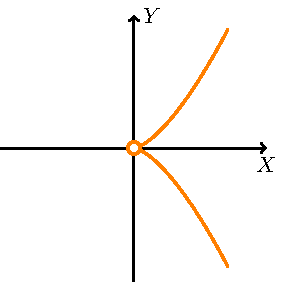
\includegraphics{Curve1.pdf}
		
		$Y^2=X^3$
	\end{minipage}
	\begin{minipage}{0.42\textwidth}
		\centering
		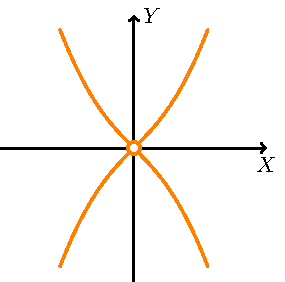
\includegraphics{Curve2.pdf}
		
		$Y^2=X^4+X^2$
	\end{minipage}
\end{center}

		
\begin{rem*}
    By Proposition~\reff{prop:dimLeqGeneratorsMaximal} and the proof of Proposition~\reff{prop:Jacobian}, 
    \begin{align*}
        \dim\left\{\nabla f(x)\st f\in\pp\right\} \leq \codim(X,k^n)\;.
    \end{align*}
\end{rem*}
\begin{rem}
    The $k$-vector space $\Nn = \left\{\nabla f(x) \st f\in \pp\right\}$ may be viewed as the \emph{conormal space} to $X$ at $x$ (at least if $X$ is regular at $x$) and its complement 
    \begin{align*}
        \Nn^\perp = \left\{ \xi = (\xi_i)_{i=1}^n \in k^n \st \sum_{i=1}^{n}\frac{\partial f}{\partial X_i}(x)\cdot\xi_i=0 \text{ for all } f\in \pp\right\}
    \end{align*}
    as the \emph{tangent space} at $x$ of $X$.
\end{rem}
\begin{thm}\lbl{thm:codimIneqRegular}
    Let $X\subseteq k^n$ be quasi-affine and $Y,Z \subseteq X$ be irreducible closed subsets and $C$ be any irreducible component of $Y\cap Z$. If there is at least one point $x\in C$ such that $X$ is regular at $x$, then 
    \begin{align*}
    	\codim(C,X) \leq \codim (Z,X)+\codim(Y,X)\;.
    \end{align*}
\end{thm}
\begin{rem}
    Let $n=4$, identify $k^4$ with the space of $2\times 2$-matrices and let $X= \left\{ A\st \det A = 0\right\}$. This has dimension 3 (where $X$ turns out to be irreducible), and 
    \begin{align*}
        Y = \left\{\begin{pmatrix} a&b\\ 0&0\end{pmatrix} \st a,b\in k \right\}\;,\quad
        Z = \left\{\begin{pmatrix} 0&0\\ c&d\end{pmatrix} \st c,d\in k \right\}
    \end{align*}  
    are irreducible closed subsets of codimension 1 and (thus) dimension 2. But $Y\cap Z = \{0\}$ has codimension 3 in $X$.
\end{rem}
\begin{proof}[Proof of Theorem \reff{thm:codimIneqRegular}]
	First of all, passing to the respective closures (which doesn't change codimension, e.g. by the \emph{locality of codimension}, cf. Remark~\reff{rem:proofPreparations}\itememph{a}), we may assume that $X,Y,Z$ are affine.
	
    \emph{Step 1.} As in the proof of Theorem~\reff{thm:codimIneq}, let $\Delta$ be the diagonal in $k^{2n}$. We will show the following: If $f_1,\ldots, f_d\in\Oo_{X,x}$ generate the maximal ideal $\mm_{X,x}$ of $\Oo_{X,x}$, then there exists an affine open neighbourhood $U$ of $x$ in $X$ and preimages of the $f_i$ in $\Oo(U)$ (which we will also call $f_i$) such that 
    \begin{align}\lbl{eq:conditionOnUxU}
        \Delta \cap (U\times U) = \left\{(y,z)\in U\times U \st f_i(y) = f_i(z) \text{ for } 1\leq i \leq d\right\}= V(g_1,\ldots,g_d)\tag{$*$}
    \end{align}
    (where $g_i(y,z)=f_i(y)-f_i(z)$), possibly after shrinking $U$. As $U$ is required to be \emph{affine open}, i.e. $U=X\setminus V(h)$ for some $h\in\Oo(X)$, we obtain that $Y\cap U=Y\setminus V(h|_Y)\eqqcolon Y'$ and $Z\cap U=Z\setminus V(h|_Z)\eqqcolon Z'$ are affine open as well, hence isomorphic to affine varieties (\cite[Proposition~2.2.4]{alg1}) and it makes sense to talk about vanishing sets of regular functions on $Y'$ and $Z'$ -- which we will do now. 
    
    Consider $\gamma_1,\ldots, \gamma_d\in\Oo(Y'\times Z')$, $\gamma_i(y,z)=f_i|_{Y'}(y)-f_i|_{Z'}(z)$ (this essentially restricts $g_1,\ldots, g_d$ to $Y'\times Z'$). We identify $Y\cap Z$ with $\Delta\cap (Y\times Z)$ and thus $C$ with its respective image, as we did in the proof of Theorem~\reff{thm:codimIneq}. Hence $C$ is an irreducible component of $\Delta\cap (Y\times Z)$. Then $C'=C\cap (U\times U)$ is an irreducible component of $\Delta\cap (Y'\times Z')=V(\gamma_1,\ldots,\gamma_d)$ (here we used \eqreff{eq:conditionOnUxU}) and Theorem~\reff{thm:krullIdeal} together with \emph{locality of codimension} yields
    \begin{align*}
    	\codim(C,Y\times Z)=\codim(C',Y'\times Z')\leq d\;.
    \end{align*}
    We silently went over an important detail: $U\times U\subseteq X\times X$ is open again. This is easily seen as $(X\setminus U)\times X$ and $X\times (X\setminus U)$ are closed (using e.g. the argument from the proof of Proposition~\reff{prop:codimensionProduct}), but don't be fooled: this \emph{does not} follow from \emph{product topology stuff}; the Zariski topology on $k^{2n}$ and $X\times X$ is \emph{not} the product of the Zariski topologies on $k^n$ or $X$. 
    
    Enough of that. From Proposition~\reff{prop:codimensionProduct} we get
    \begin{align*}
    	\codim(Y\times Z,X\times X)&=\dim(X\times X)-\dim(Y\times Z)=(\dim X-\dim Y)+(\dim X-\dim Z)\\
    	&=\codim(Y,X)+\codim(Z,X)
    \end{align*}
    and hence, 
    \begin{align*}
        \codim(C,X)& = \dim(X) -\dim(C)\\
        &= \dim (X) - (\dim(X)+\dim(X) -\codim(C,X\times X))\\
        &= \codim(C,X\times X) -\dim X\\
        &=\codim(C,Y\times Z)+\codim(Y\times Z,X\times X)-\dim X\\
        &\leq \codim(Y,X) +\codim(Z,X) +d-\dim(X) \\
        &=\codim(Y,X) +\codim(Z,X),
    \end{align*}
    provided that $d=\dim(X)$, which is possible for an appropriate choice of the $f_i$ when $X$ is regular at $x$ (by \NAK, $\mm_{X,x}$ can be generated by $\dim X$ elements, cf. the proof of Proposition~\reff{prop:dimLeqGeneratorsMaximal} or \cite[Concluding remarks, Lemma~1\itememph{c}]{alg1}).
    
    \emph{Step 2.} Let $R= k[X_1,\ldots, X_m]$ and $\pp,\mm\subseteq R$ be the prime ideal defining $k^\ell \times \{0\}^{m-\ell}$ respectively the maximal ideal defining $\{0\}^m$. Then $\mm^2 \cap \pp \subseteq \mm\cdot\pp$. This can be shown as follows. Since $\mm$ is generated by $X_1,\ldots,X_m$, $\mm^2$ is generated by the $X_iX_j$ (with $i,j$ not necessarily distinct). Similarly, $\pp$ is the ideal generated by $X_{\ell+1},\ldots, X_m$. If $f\in R$ lies in both $\mm^2$ and $\pp$, each monomial of $f$ must be divisible by some $X_iX_j$ as well as by some $X_{\ell+r}$. Then this monomial is divisible by $X_iX_{\ell+r}$ or $X_jX_{\ell+r}$, hence contained in $\mm\cdot\pp$. Now $f\in\mm\cdot\pp$ because each monomial lies in that ideal.
       
   \emph{Step 3.} Let $\xi\in k^m$, $L\subseteq k^m$ an affine subspace containing $\xi$. Let $\pp$ be the prime ideal defining $L$ and $\mm$ the maximal ideal defining $\{\xi\}$. Then $\pp\cap \mm^2 \subseteq I\cdot \mm$. This can be reduced to the previous step by an affine automorphism of $k^m$.
    
    \emph{Step 4.} Let $x\in k^n$, $\mm_x \subseteq S= k[X_1,\ldots, X_n]$ the maximal ideal defined by $x$, $f_1,\ldots, f_n\in S$ such that their images generate $\mm_x/\mm_x^2$. Then there is $h\in R = k[X_1,\ldots, X_n,Y_1,\ldots Y_n]$ such that $h(x,x) \neq 0$ and $h\cdot \pp_\Delta \subseteq (g_1,\ldots, g_n)_R$ where $g_i(y,z) = f_i(y)-f_i(z)$ and $\pp_\Delta\subseteq R$ is the prime ideal of functions vanishing on $\Delta = \left\{(y,y)\st y\in k^n\right\}$. To see this, let $\xi = (x,x)$ and $\qq = \pp_\Delta \cdot R_{\mm_\xi}$, where $\mm_\xi\subseteq R$ denotes the maximal ideal of functions vanishing on $\xi$. Let $\nn = \mm_\xi\cdot R_{\mm_\xi}$ denote the maximal ideal of the local ring $R_{\mm_\xi}$. From the previous step it follows that 
    \begin{align}\lbl{eq:thm15}
        \nn^2\cap \qq\subseteq \qq\cdot \nn .
    \end{align}
    Let $\gg\subseteq \qq$ be the ideal generated by the images of the $g_i$. Our long-term goal is to show $\gg=\pp$. Let $f\in \pp_\Delta$. We claim that there are $c_1,\ldots,c_n$ such that $g=f-\sum_{i=1}^n c_i g_i$ is in $\mm_\xi^2$. Indeed, by the isomorphism \eqreff{eq:modToNabla} this is equivalent to $\nabla g(\xi)=0$. Since $f|_\Delta = 0$, we have $\frac{\partial f}{\partial X_i}(\xi) + \frac{\partial f}{\partial Y_i}(\xi) = 0$ at $\xi\in \Delta$ and the same for the $g_i$. Thus, it is sufficient to have 
    \begin{align*}
        \frac{\partial f}{\partial X_i}(\xi) = \sum_{j=1}^n c_j \frac{\partial g_j}{\partial X_i}(\xi) = \sum_{j=1}^n c_j \frac{\partial f_j}{\partial X_i}(x)\quad\text{for all }i=1,\ldots,n
    \end{align*}
    (the second equality is tautological), which is possible since the $f_i$ generate $\mm_x/\mm_x^2$, hence the $\nabla f_i(x)$ generate $k^n$ by the isomorphism \eqreff{eq:modToNabla}. It follows that $\pp_\Delta\subseteq (g_1,\ldots,g_n)_R + (\pp_\Delta\cap \mm_\xi^2) = (g_1,\ldots,g_n) + \pp_\Delta\cdot \mm_\xi$ (the second equality follows from Step 3). This is still true in the localization at $\mm_\xi$, i.e. $\qq\subseteq \gg +\qq\cdot\nn$. By Corollary \reff{cor:NAK}, we have $\qq= \gg$. 
    
    Now let $\phi_1,\ldots,\phi_N$ generate $\pp_\Delta$. Since $\qq =\pp_\Delta\cdot R_{\mm_\xi}$ is generated by the images of the $g_i$, there are $h_i\not\in \mm_\xi$ and such that $h_i\cdot \phi_i \in(g_1,\ldots,g_n)_R$. Then $h=h_1\cdots h_N$ fulfills $h(\xi)=h(x,x)\not=0$ and $h\cdot\pp_\Delta\subseteq(g_1,\ldots,g_n)_R$.
    
    \emph{Step 5.} Let $f_1,\ldots, f_d$ be elements of $S= k[X_1,\ldots, X_n]$ such that their images in $\Oo_{X,x}$ form a base of $\mm_{X,x}/\mm_{X,x}^2$ (again, $\mm_{X,x}$ is the maximal ideal of the local ring $\Oo_{X,x}$, which Professor Franke would like to express as $\mm_{X,x}=\rad \Oo_{X,x}$). Let $f_{d+1},\ldots, f_n$ be chosen in such a way that the images of $f_1,\ldots, f_n$ form a base of $\mm_x/\mm_x^2$. Why is this possible? We have $\mm_{X,x}/\mm_{X,x}^2=\nn/\nn^2$, $\nn\subseteq\Oo(X)$ denoting the maximal ideal of $\Oo(X)$ of functions vanishing at $x$. Then $\nn/\nn^2$ is a quotient of $\mm_x/\mm_x^2$ (as we saw in the proof of Proposition~\reff{prop:Jacobian}). If $h$ is as in the previous step, $U= X\setminus V(h)$ has the required property.
\end{proof}
\begin{rem}[on \eqreff{eq:thm15}]
    Let $R$ be an arbitrary ring, $S\subseteq R$ a multiplicative subset, $I$ and $J$ ideals in $R$. Then 
    \begin{align*}
        (I+J) \cdot R_S &= I\cdot R_S + J \cdot R_S\\
        (I\cap J)\cdot R_S &= I\cdot R_S \cap J\cdot R_S\\
        (I\cdot J)\cdot R_S &= (I\cdot R_S)\cdot(J\cdot R_S)\\
        \sqrt{I\cdot R_S}&= \sqrt{I}\cdot R_S
    \end{align*}
\end{rem}
\begin{proof}
    We will only prove the second equality, they are all quite similar. The image of $I\cap J$ is contained in both $I\cdot R_S$ and $J\cdot R_S$, hence so is $(I\cap J)\cdot R_S$, proving $(I\cap J) \cdot R_S \subseteq I\cdot R_S \cap J\cdot R_S$. Conversely, let $\rho \in (I \cdot R_S)\cap (J\cdot R_S)$. Since $\rho\in I\cdot R_S$, $\rho = \frac{i}{s}$ where $i\in I$ and $s\in S$. Since $\rho\in J\cdot R_S$, $\rho = \frac{j}{t}$ where $j\in J$ and $t\in S$. Since $\frac{i}{s}=\frac{j}{t}$ in $R_S$, there is $\sigma \in S$ such that $\sigma i t = \sigma  j  s$. Then $\rho = \frac{\sigma  i t}{\sigma  s t} = \frac{\sigma  j s}{\sigma  s t}\in (I\cap J)\cdot R_S$.
\end{proof}



\section{Derivations and the module of Kähler differentials}
\begin{defi}[Derivations]\lbl{def:derivation}
    Let $A$ be a ring, $M$ an $A$-module, $d\colon A\to M$  a homomorphism of the additive group. We say that $d$ is a \defemph{derivation} of $A$ with values in $M$ if it satisfies the \emph{Leibniz rule} 
    \begin{align*}
    	 d(a\cdot b) = b\cdot d(a) + a\cdot d(b)\;.
    \end{align*}
     If $A$ is an $R$-algebra and $A\morphism[d] M$ a derivation of $A$, we call $d$ \emph{$R$-linear} if the following equivalence conditions hold:
    \begin{alphanumerate}
        \item 
            $d(r) = 0$ for all $r\in R$.
        \item
            $d(r\cdot a) = r\cdot d(a)$ for all $r\in R, a\in A$.
    \end{alphanumerate}
    Let $\Der(A,M)$ denote the set of derivations with values in $M$. This can be given a canonical $A$-module structure via $(a\cdot d)(b) = a\cdot d(b)$.
\end{defi}
\begin{proof}
    Let $d\in \Der(A,M)$. Note that we always have $d(1)=0$ as $d(1)=d(1\cdot1)=d(1)+d(1)$ by the Leibniz rule. Now, assuming $d(r\cdot a)=r\cdot d(a)$ for all $r\in R, a\in A$, we obtain $d(r)=d(r\cdot1)=0$. Conversely, if $d(r)=0$ for all $r\in R$, then $d(a\cdot r) = a\cdot d(r) + r\cdot d(a) = r\cdot d(a)$ by the Leibniz rule. Hence, \itememph{a} and \itememph{b} are indeed equivalent.
\end{proof}
\begin{rem}
    The set $\Der_R(A,M)$ of $R$-linear derivations forms an $A$-submodule of $\Der(A,M)$.
\end{rem}
\begin{example}\lbl{ex:universalDerivationPolynomialRing}
    A derivation $d\in\Der_R(R[X_1,\ldots,X_n], M)$ is uniquely determined by the tuple $(m_1,\ldots,m_n)\in M^n$ via
    \begin{align*}
        d&\longmapsto (dX_1,\ldots,dX_m)\\
        \bigg(P\mapsto \sum_{i=1}^n\frac{\partial P}{\partial X_i}\cdot m_i \bigg) &\longmapsfrom (m_1,\ldots,m_n)\;.
    \end{align*}
    Note that the left hand side is indeed a derivation:
    \begin{align*}
        d(PQ) = \sum_{i=1}^n \frac{\partial(PQ)}{\partial X_i} \cdot m_i = \sum_{i=1}^n \left( P \cdot\frac{\partial Q}{\partial X_i} + Q\cdot\frac{\partial P}{\partial X_i} \right) m_i = P\cdot d(Q) + d(P)\cdot Q\;.
    \end{align*}
    It is easy to see that the two maps are inverse to each other.
\end{example}
\begin{rem*}
    $\Der(A,-)$ and $\Der_R(A,-)$ are functors: If $M\morphism[\mu] N$ is a homomorphism of $A$-modules then 
    \begin{align*}
        \Der(A,M) &\longto \Der(A,N)\\
        d &\longmapsto \mu \circ d
    \end{align*}
    is a morphism of $A$-modules and similar for $\Der_R(A,M)$ and $\Der_R(A,N)$.
    
    The previous Example~\reff{ex:universalDerivationPolynomialRing} can be re-formulated as saying that
    \begin{align*}
        d\colon A = R[X_1,\ldots, X_n] &\longto A^n\\
        P &\longmapsto \nabla P=\bigg(\frac{\partial P}{\partial X_1},\ldots,\frac{\partial P}{\partial X_n}\bigg)
    \end{align*}
    is the \emph{universal} $R$-linear derivation of $A$: Any $\delta \in \Der_R(A,M)$ can be uniquely expressed as $\delta = \mu \circ d$ where $A^n \morphism[\mu] M$ is a uniquely determined $A$-linear homomorphism.
\end{rem*}
\begin{defi}[Kähler differentials] \lbl{def:KahlerDiff}
    Let $A$ be an $R$-algebra. A \defemph{module of Kähler differentials} for $A/R$ is an $A$-module $\Omega_{A/R}$ together with $d_{A/R} \in \Der_R(A,\Omega_{A/R})$ satisfying the following universal property: 
    \begin{quote}
    	For any $A$-module $M$ and any $\delta \in \Der_R(A,M)$ there is a unique $A$-homomorphism $\Omega_{A/R}\morphism[\epsilon] M$ such that
    	\begin{diagram}
    		\node (A) at (0,1.25) {$A$};
    		\node (M) at (2.5,1.25) {$M$};
    		\node (O) at (1.25,0) {$\Omega_{A/R}$};
    		\scriptsize
    		\draw[->] (A) -- (M) node[pos=0.5, above] {$\delta$};
    		\draw[->] (A) -- (O) node[pos=0.5, below left] {$d_{A/R}$};
    		\draw[->, dashed] (O) -- (M) node[pos=0.5, below right] {$\exists!\ \epsilon$};
    	\end{diagram}
    \end{quote}
     It is worth pointing out that we thus defined $\Omega_{A/R}$ by an \emph{$(\epsilon,\delta)$-definition}!
\end{defi}
\begin{rem*}
    \begin{alphanumerate}
        \item 
            The universal property characterizes $\Omega_{A/R}$ up to unique isomorphism (if it exists): If $\snake d_{A/R} \in\Der_R(A,\snake \Omega_{A/R})$ has the same universal property, there is a unique isomorphism $\Omega_{A/R}\isomorphism[i] \snake \Omega_{A/R}$ such that $\snake d _{A/R} = i \circ d_{A/R}$. In fact, the universal property of $d_{A/R}$ shows the existence and uniqueness of a homomorphism $i$ with this property. Reversing the roles of $d_{A/R}$ and $\snake d_{A/R}$ we also obtain $\snake\Omega_{A/R} \morphism[j]\Omega_{A/R}$ such that $d_{A/R} = j\circ \snake d_{A/R}$. Then $\alpha = j\circ i$ satisfies $d_{A/R} = \alpha\circ d_{A/R}$ which implies $\alpha= \id_{\Omega_{A/R}}$ by the universal property of $\Omega_{A/R}$. Exchanging $d_{A/R}$ and $\snake d_{A/R}$ gives $i \circ j = \id_{\snake\Omega_{A/R}}$. Thus, $i$ is an isomorphism.
        \item
            For $A= R[X_1,\ldots,X_n]$, $\Omega_{A/R} = \bigoplus_{i=1}^n A\cdot dX_i \simeq A^n$ with $d_{A/R} (P) = \sum_{i=1}^n \frac{\partial P }{\partial X_i} \cdot dX_i$ is a module of Kähler differentials.
        \item 
            If $A$ is a quotient of $R$ (i.e. $R\morphism A$ is surjective) then $\Der_R(A,M) = 0$ for all $M$, hence $\Omega_{A/R} = 0$.
    \end{alphanumerate}
\end{rem*}
\begin{defi}[Free module] \lbl{def:freeModule}
    The free $A$-module $F$ with generating set $M$, $F=\bigoplus_{m\in M}A$, is the $A$-module of functions $f\colon M \morphism A$ with finite support. We define $\delta_x \in F$ by $\delta_x(y) = \delta_{x,y}$ (i.e. $\delta_x(x)=1$ and $\delta_x(y)=0$ for $y\not=x$).
\end{defi}

\begin{rem*}
    \begin{alphanumerate}
        \item  
            One often thinks of $F$ as the module of formal (finite) $A$-linear combinations of $M$ with $f=\sum_{x\in M} f(x) x$ instead of $f= \sum_{x\in M} = f(x)\delta_x$.
        \item 
            We have a bijection, for any $A$-module $N$,
            \begin{align*}
                \Hom_{\cat{Set}}(M,N) &\isomorphism \Hom_A(F,N)\\
                \upsilon &\longmapsto \bigg(f\mapsto \sum_{m\in M} f(m) \upsilon(m)\bigg)\\
                \big(m\mapsto \phi(\delta_m) \big) &\longmapsfrom \phi\;.
            \end{align*}
            In other words, mapping $X$ to the free $A$-module generated by $X$ as a functor from $\cat{Set}$ to the category of $A$-modules is \emph{left-adjoint} to the forgetful functor from the category of $A$-modules to $\cat{Set}$.
    \end{alphanumerate}
\end{rem*}

\begin{prop}\lbl{prop:kahlerExists}
    A module $\Omega_{A/R}$ of Kähler differentials  exists for any $R$-algebra $A$.
\end{prop}
\begin{proof}
    %If $(A\morphism[d] M) \in \Der_R(A,M)$ it defines a unique $F_A\morphism[c] M$ where $F_A$ is the free $A$-module generated by $A$, such that $d(a) = c(\delta_a)$.
    We follow the \emph{brute-force} approach to constructing $\Omega_{A/R}$. Let $F_A$ be the free $A$-module generated by the set $A$ itself and let $K\subseteq F_A$ the submodule generated by the following three types of elements:
    \begin{alphanumerate}
        \item 
            $\left\{\delta_x+\delta_y-\delta_{x+y}\st x,y\in A\right\}$
        \item 
            $\left\{\delta_r\st r\in R\right\}$
        \item 
            $\left\{x\delta_y+y\delta_x -\delta_{xy} \st x,y\in A\right\}$
    \end{alphanumerate}
    Let $\Omega_{A/R} = F_A/K$, $F\morphism[\pi] \Omega_{A/R}$ be the projection to the quotient and put $d_{A/R}(a) = \pi(\delta_a)$. It is easy to see that $d_{A/R}\in \Der_R(A,M)$ e.g.
    \begin{align*}
        d_{A/R}(ab) = \pi(\delta_{ab}) = \pi(\delta_{ab}-a\delta_b -\delta_a) + a\pi(\delta_b) +b\pi(\delta_a) = a\cdot d_{A/R}(b) + b\cdot d_{A/R}(a)
    \end{align*}
    as $\delta_{ab}-a\delta_b -\delta_a\in K$ and by the definition of $d_{A/R}$.
    
    Let $(A\morphism[d] M)\in \Der_R(A,M)$. By the universal property of $F_A$ there is a unique morphism $c\in \Hom_A(F_A,M)$ such that $d(a) = c(\delta_a)$. We claim that $c$ vanishes on $K$.
    \begin{itemize}
      \item 
        $c(\delta_a +\delta_b -\delta_{a+b}) = c(\delta_a) +c(\delta_b) -c(\delta_{a+b}) = d(a)+d(b)-d(a+b) = 0$ as $d$ is additive.
      \item 
        $c(\delta_r) = d(r) = 0$ when $r\in R$ as $d$ is $R$-linear.
      \item 
        $c(a\delta_b+b\delta_a -\delta_{ab}) = a\cdot d(b) + b\cdot d(a) - d(ab) = 0$ by the Leibniz rule.
    \end{itemize}
    Consequently, due to the universal property of quotient modules, there is a unique $\delta\in \Hom_A(F_A/K , M)$ such that 
    \begin{diagram}
    	\node (FA) at (0,1.25) {$F_A$};
    	\node (M) at (2.5,1.25) {$M$};
    	\node (O) at (1.25,0) {$F_A/K$};
    	\scriptsize
    	\draw[->] (FA) -- (M) node[pos=0.5, above] {$d$};
    	\draw[->] (FA) -- (O) node[pos=0.5, below left] {$\pi$};
    	\draw[->, dashed] (O) -- (M) node[pos=0.5, below right] {$\exists!\ \delta$};
    \end{diagram}
    commutes. Therefore, $F_A/K=\Omega_{A/R}$ satisfies the universal property.
\end{proof}
In many cases, the module of Kähler differentials can be calculated using $\Omega_{R[X_1,\ldots,X_n]}\simeq \bigoplus_{i=1}^n R[X_1,\ldots, X_n] dX_i$ and two exact sequences which follow in a straight forward way from
\begin{fact}\lbl{fact:DerExactSequences}
    Let $R$ be a ring, $A$ an $R$-algebra.
    \begin{alphanumerate}
        \item 
            Let $I\subseteq A$ be any ideal, $M$ any $A/I$-module, $A\morphism[\pi]A/I$ the projection, then 
            \begin{align}\lbl{eq:derExactSequence1}
                0\morphism \Der_R(A/I,M) \morphism \Der_R(A,M) \morphism \Hom_{A/I}(I/I^2, M) 
            \end{align}
            is exact. Herein, the morphism $\Der_R(A/I,M) \morphism \Der_R(A,M)$ is defined by $d\mapsto \delta=d\circ\pi$ and $\Der_R(A,M) \morphism \Hom_{A/I}(I/I^2, M)$ by $\delta\mapsto\phi = \left(i\mod I^2\mapsto\delta(i)\right)$.
        \item 
            Let $B$ be an $A$-algebra, $M$ an $B$-module, then we have the exact sequence
            \begin{align}\lbl{eq:derExactSequence2}
	            \begin{split}
		            0 \morphism \Der_A(B,M) \monomorphism\Der_R(B,M) &\morphism \Der_R(A,M)\\
		            d&\longmapsto d|_A\;.
	            \end{split}
            \end{align}
    \end{alphanumerate}
\end{fact}
\begin{proof}
    We will first proof \itememph{b}. The exactness on the left end is obvious, as is the vanishing of the composition $\Der_A(B,M) \monomorphism \Der_R(B,M) \morphism \Der_R(A,M)$. Let $d\in \Der_R(B,M)$ such that $0 = d|_A$, then $d$ is $A$-linear, i.e. $d\in \Der_A(B,M)$.
    
    Now about \itememph{a}. That $\Der_R(A/I,M) \morphism \Der_R(A,M)$ is well-defined is obvious, as derivations are compatible with applying ring homomorphisms on the right. To show that the rightmost arrow is well-defined, we first need to show that $\delta\in\Der_R(A,M)$ vanishes on $I^2$. If $i,j\in I$, then $\delta(i\cdot j)=i\cdot\delta(j)+j\cdot\delta(i)=0$ as $I\cdot M=0$, hence $\delta$ indeed vanishes on $I^2$ as $I^2$ is generated by the $ij$ where $i,j\in I$. It follows that $\phi$ is indeed a homomorphism of abelian groups. Let $\alpha = a\mod I\in A/I$ and $i\in I$, then $\phi(\alpha \cdot (i\mod I^2)) = \delta(a\cdot i) = i\cdot \delta(a) + a\cdot \delta(i) = \alpha\cdot\delta(i)$ showing that $\phi$ is $(A/I)$-linear as stated. 
    
    Exactness on the left end follows from the surjectivity of $A\morphism[\pi] A/I$. The fact that the composition $d\in\Der_R(A/I,M)\mapsto\delta\in\Der_R(A,M)\mapsto\phi\in\Hom_{A/I}(I/I^2,M)$ is zero is also obvious: $\phi(i\mod I^2) = \delta(i) = d(\pi(i)) = d(0) = 0$. Finally, let $\delta$ be such that $\phi = 0$. For $i\in I$, $\delta(i) = \phi(i\mod I^2) = 0$. Hence there exists a unique group homomorphism $A/I \morphism[d] M$ such that $\delta = d\circ \pi$. The Leibniz rule for $d$ follows from the analogous rule for $\delta$ and the surjectivity of $\pi$.
\end{proof}
\begin{fact*}\lbl{fact:HomRightExact}
    Let $A$ be any ring, $M'\morphism M\morphism M''\morphism 0$ a sequence of $A$-homomorphisms, then this sequence is exact iff $0\morphism\Hom_A(M'',T) \morphism \Hom_A(M,T) \morphism\Hom_A(M',T)$ is exact for any $A$-module $T$.
\end{fact*}
\begin{cor}\lbl{cor:kahlerExactSequences}
    Let $R$ be a ring, $A$ an $R$-algebra. 
    \begin{alphanumerate}
        \item 
            If $I\subseteq A$ is any ideal, we have a canonical short exact sequence of $(A/I)$-modules
            \begin{align}\lbl{eq:tensorDerSpam1}
                I/I^2\morphism[\alpha] \Omega_{A/R} \otimes_A A/I \morphism[\beta] \Omega_{(A/I)/R} \morphism 0\;.
            \end{align}
        \item 
            If $B$ is any $A$-algebra, we have a canonical short exact sequence of $B$-modules
            \begin{align}\lbl{eq:tensorDerSpam2}
                \Omega_{A/R}\otimes_A B \morphism[\kappa] \Omega_{B/R} \morphism[\lambda] \Omega_{B/A} \morphism 0\;.
            \end{align}
    \end{alphanumerate}
\end{cor}
\begin{rem*}
    \begin{alphanumerate}
        \item 
            Tensor products as occuring above are used for change of base: $M\otimes_A B$ is a $B$-module together with a morphism $M\morphism M\otimes_A B$, $m \mapsto m \otimes_A 1$ with the following universal property: 
            \begin{quote}
            	If $T$ is any $B$-module and $M\morphism[\tau] T$ any $A$-linear homomorphism, then there is a unique homomorphism $M\otimes_A B \morphism[t] T$ such that
            	\begin{diagram}
            		\node (M) at (0,1.25) {$M$};
            		\node (T) at (2.5,1.25) {$T$};
            		\node (MB) at (1.25,0) {$M\otimes_AB$};
            		\scriptsize
            		\draw[->] (M) -- (T) node[pos=0.5, above] {$\tau$};
            		\draw[->] (M) -- (MB) node[pos=0.5, below left] {$-\otimes_A1$};
            		\draw[->, dashed] (MB) -- (T) node[pos=0.5, below right] {$\exists!\ t$};
            	\end{diagram}
            	 commutes, i.e. $\tau(m) = t(m\otimes_A 1)$. In particular, there is an isomorphism $\Hom_A(M,T)\simeq\Hom_B(M\otimes_AB,T)$ of $B$-modules.
            \end{quote}
            For instance, $V\otimes_\IR \IC$ is the complexification of the $\IR$-vector space $V$. We put $m\otimes_A b= b\cdot (m\otimes_A 1)$. One easy special case is $B=A/I$ in which case 
            \begin{align*}
            	M\otimes_A(A/I)=M/(I\cdot M)\;, \quad m\otimes_A (a\mod I) \coloneqq (a\cdot m) \mod (I \cdot M)
            \end{align*}
            has the desired universal property.
        \item
            Using and \reff{eq:tensorDerSpam1} the calculation of $\Omega_{R[T_1,\ldots,T_n]/R}$ it is possible to calculate $\Omega_{(A/I)/R}$ (where $A=R[T_1,\ldots, T_n]$) as the cokernel of 
            \begin{diagram}
            	\node (I) at (0,1.25) {$I/I^2$};
            	\node (O) at (2,1.25) {$\Omega_{A/R}\rlap{$/(I\cdot\Omega_{A/R})$}$};
            	\node (A) at (2, 0) {$(A/I)^n$};
            	\path (A) -- (O) node[pos=0.5, sloped] {$\simeq$};
            	\scriptsize
            	\path (I) ++ (-1.75,-0.25) node (i) {$f\mod I^2$};
            	\path (A) ++ (-1.75,-0.25) node (a) {$\nabla f\mod I$};
            	\draw[->] (I) -- (O);
            	\draw[->] (I) -- (A);
            	\draw[|->] (i) -- (a);
            \end{diagram}
            Since any $R$-algebra of finite type has the form $A/I$, this provides a way to calculate $\Omega_{B/R}$ for such $R$-algebras $B$. Since Example \reff{ex:universalDerivationPolynomialRing} is not (really) limited to case of finitely many variables, other $R$-algebras could be treated as well.
    \end{alphanumerate}
\end{rem*}
\begin{proof}[Proof of Corollary~\reff{cor:kahlerExactSequences}]
	Let us first construct the involved canonical homomorphisms.
	\begin{itemize}
		\item 
		By the universal property of $d_{B/R}$, the derivation $d_{B/A}\colon B\morphism \Omega_{B/A}$ (which is $R$-linear) hence has a unique representation 
		\begin{align*}
			d_{B/A} = \lambda \circ d_{B/R}\;,
		\end{align*}
		in which $\lambda$ is an $B$-homomorphism $\Omega_{B/R}\morphism[\lambda]\Omega_{B/A}$.
		 \item 
		 Composing $d_{B/R}\colon B \morphism \Omega_{B/R}$ with $A\morphism B$ gives us an element of $\Der_R(A, \Omega_{B/R})$, which, by the universal property of $\Omega_{A/R}$, is given by a unique $A$-module-homomorphism 
		 \begin{align*}
		 	\Omega_{A/R} \morphism[\kappa'] \Omega_{B/R}\;.
		 \end{align*}
		 By the universal property of $-\otimes_A B$, $\kappa'$ is given by a unique $B$-module-homomorphism
		 \begin{align*}
		 	\Omega_{A/R} \otimes_A B \morphism[\kappa] \Omega_{B/R}\;.
		 \end{align*}
		 In other words, $\kappa$ is the unique $B$-module-homomorphism such that $\kappa(d_{A/R}(a)\otimes_A b) = b\cdot d_{B/R}(a)$.
		 \item 
		 The $A/I$-homomorphism $\beta$ is uniquely determined by 
		 \begin{align*}
		 	\beta\left(d_{A/R}(a) \mod (I\cdot \Omega_{A/R})\right) = d_{(A/I)/R}(a)\;.
		 \end{align*}
		 In other words, this is the special case $B=A/I$ of $\kappa$.
		 \item 
		 We put 
		 \begin{align*}
		 	\alpha(i\mod I^2) = d_{A/R}(i) \mod (I\cdot \Omega_{A/R})\;.
		 \end{align*}
		 In other words, $\alpha$ is obtained by applying $\Der_R(A,M) \morphism \Hom_{A/I} (I/I^2, M)$ from Fact~\reff{fact:DerExactSequences} to the derivation $A\xrightarrow{\smash{d}_{A/R}} \Omega_{A/R} \morphism \Omega_{A/R}/I \cdot \Omega_{A/R} \eqqcolon M$.
	\end{itemize}
	It remains to show exactness. By \hyperref[fact:HomRightExact]{this} unnamed fact, it is sufficient to show that exactness holds after applying the functor $\Hom_B(-,T)$ for any $B$-module $T$ (where in \itememph{a} we have the special case $B=A/I$). Note that 
	\begin{align*}
		\Hom_A\left(\Omega_{A/R},T\right)\simeq\Der_R(A,T)\quad\text{and}\quad \Hom_B\left(\Omega_{A/R}\otimes_AB,T\right)\simeq \Hom_A\left(\Omega_{A/R},T\right) 
	\end{align*}
	by the universal properties of $\Omega_{A/R}$ and $-\otimes_AB$. Hence, applying $\Hom_B(-,T)$ transforms \eqreff{eq:tensorDerSpam1} and \eqreff{eq:tensorDerSpam2} into \eqreff{eq:derExactSequence1} and \eqreff{eq:derExactSequence2} respectively, thus showing exactness by Fact~\reff{fact:DerExactSequences}.
\end{proof}









\appendix
\chapter{Appendix}
\setcounter{thm}{0}
\renewcommand*{\thethm}{\Alph{thm}}
\section{Introduction to Krull dimension and all that}
Professor Franke recapitulated on some topics of his previous lecture, Algebra I (of which detailed lecture notes may be found in \cite{alg1}). Note that although the numbering of theorems in the following might seem messy, it is \emph{intentionally} messy at least.
\begin{defi}[{\cite[Definition~2.1.2]{alg1}}]
	A topological space $X$ is called \defemph{quasi-compact} if every open cover $X = \bigcup_{\lambda\in\Lambda} U_\lambda$ admits a finite subcover.
	
	$X$ is \defemph{Noetherian} if it satisifies the following equivalent conditions:
	\begin{alphanumerate}
		\item Every open subset is quasi-compact.
		\item There is no infinite properly descending chain of closed subsets.
		\item Every set of closed subsets of $X$ has a $\subseteq$-minimal element.
	\end{alphanumerate}
\end{defi}

\begin{defi}[{\cite[Definition~2.1.3]{alg1}}]
	A topological space $X\not=\emptyset$ is \defemph{irreducible} if it satisifies the following equivalent conditions:
	\begin{alphanumerate}
		\item If $X = X_1\cup X_2$ where $X_1$ and $X_2$ are closed subsets, then $X=X_1$ or $X=X_2$. Also, $X\neq\emptyset$.
		\item Any two non-empty open subsets of $X$ have non-empty intersection.
		\item Every non-empty open subset of $X$ is dense.
	\end{alphanumerate}
\end{defi}
Condition (a) implies, by induction, the following more general property: 
For any finite cover $X= \bigcup_{i=1}^n X_i$ by closed subsets, there is $1\leq i\leq n$ such that $X=X_i$.
\begin{prop}
	\begin{alphanumerate}
		\item 
		Any subset of a Noetherian topological space is Noetherian with it's induced subspace topology \emph{(cf. \cite[Remark~2.2.1]{alg1})}. \lbl{prop:irreducibleDecomposition}
		\item 
		If $X$ is Noetherian, there is a unique (that is, up to permutation of the $X_i$) decomposition $X = \bigcup_{i=1}^n X_i$ into irreducible closed subsets $X_i\subseteq X$ such that $X_i\not\subseteq X_j$ for $i\neq j$ \emph{(cf. \cite[Proposition~2.1.1]{alg1})}.
	\end{alphanumerate}
	
\end{prop}
\begin{defi}[{\cite[Definition~2.1.4]{alg1}}]
	Let $X$ be a topological space, $Z\subseteq X$ irreducible and closed. We put 
	\begin{align*}
	\codim(Z,X) &= \sup\left\{\ell\st 
	\begin{array}{c}
	\text{there is a strictly ascending chain}\\
	Z=Z_0 \subsetneq Z_1\subsetneq \ldots \subsetneq Z_\ell\subseteq X\text{ of irreducible closed }Z_i\subseteq X
	\end{array}\right\}\\
	\dim(X) &= \sup\left\{\codim(Z,X)\st Z\subseteq X \text{ irreducible and closed}\right\}
	\end{align*}
\end{defi}
\begin{example}[{\cite[Section~1.7 and 2.1]{alg1}}]\lbl{ex:vanishingSetOfIdeal}
	Let $k =\overline{k}$ be an algebraically closed field. For an ideal $I\subseteq R = k[X_1,\ldots,X_n]$ let 
	\begin{align*}
	V(I) = \left\{x\in k^n\st f(x)=0\ \forall f\in I\right\}
	\end{align*}
	be the set of zeroes of $I$. By the Hilbert Nullstellensatz, $V(I) \neq \emptyset$ when $I\subsetneq R$. Moreover 
	\begin{align*}
	V(I)& = V\left(\sqrt{I}\right)\\
	V(I\cdot J ) &= V(I) \cup V(J)\\
	V\bigg(\sum_{\lambda\in\Lambda} I_\lambda\bigg) &=\bigcap_{\lambda\in\Lambda} V(I_\lambda)\;.
	\end{align*}
	It follows that there is a topology (called the \emph{Zariski topology}) on $k^n$ containing precisely the subsets of the form $V(I)$ as closed subsets. A version of the Nullstellensatz (\cite[Proposition~1.7.1]{alg1}) says
	\begin{align*}
	\left\{f\in R\st f(x) = 0\ \forall f\in I\right\} = \left\{f\in R\st V(f)\supseteq V(I)\right\} = \sqrt{I}\;.
	\end{align*}
	This means that there is strictly antimonotonic bijective correspondence between the ideals $I$ of $R$ with $I=\sqrt{I}$ and the Zariski-closed subsets $A\subseteq k^n$ via
	\begin{align*}
	\left\{\text{ideals }I\subseteq R\text{ such that }I=\sqrt I\right\}&\isomorphism\left\{\text{Zariski-closed subsets }A\subseteq k^n\right\}\\
	\left\{f\in R\st V(f)\supseteq A\right\} &\longmapsfrom A\\
	I&\longmapsto V(I)\;.
	\end{align*}
	(cf. \cite[Remark~2.1.1]{alg1}). As $R$ is Noetherian, any strictly ascending chain of ideals in $R$ terminates, implying that $k^n$ is a Noetherian topological space. Under the above correspondence prime ideals correspond to irreducible subsets and vice versa (cf. \cite[Proposition~2.1.2]{alg1}).  
\end{example}
\begin{rem}[{\cite[Remark~2.1.3]{alg1}}]
	In general, for $A\subseteq B\subseteq C\subseteq X$
	\begin{align}\lbl{eq:codimIneq}
	\codim(A,B) +\codim(B,C) &\leq \codim(A,C) \\ 
	\codim(A,X)+\dim A &\leq \dim X.\lbl{eq:codimIneq2}
	\end{align}
	may be strict. A Noetherian topological space is called \emph{catenary} if \eqreff{eq:codimIneq} is an equality whenever $A$, $B$ and $C$ are irreducible.
\end{rem}
\begin{thm}[{\cite[Theorem~5]{alg1}}]\lbl{thm:knIsCatenary}
	The space $X=k^n$ is catenary and in this case equality always occurs in \eqreff{eq:codimIneq2}.
\end{thm}
\begin{example}
	For $n=1$, the closed subsets of $k$ are $k$ itself and the finite subsets. Since $k$ is infinite, the points and $k$ are the irreducible subsets, implying $\dim(k) = 1 $ and the other assertions for $n=1$.
\end{example}
\begin{example}
	The irreducible subsets of $k^2$ are $k^2$ itself, single points, and $V(f)$ where $f\in k[X,Y]$ is a prime element.
\end{example}
\begin{defi}[Transcendence degree]\lbl{def:degTr}
	Let $K\subseteq L$ be a field extension. A set $S\subseteq L$ is called \emph{algebraically independent} over $K$ if for all polynomials $P\in K[X_1,\ldots,X_n]$ and pairwise different $s_1,\ldots, s_n\in S$, 
	\begin{align*}
	P(s_1,\ldots, s_n) =0\quad\text{implies}\quad P=0\;. 
	\end{align*}
	A \emph{transcendence basis} of $L/K$ is a subset $S\subseteq L$ which is algebraically independent over $K$ and such that $L/K(s_1,\ldots,s_n)$ is algebraic. The \defemph{transcendence degree} $\deg\tr L/K$ of $L/K$ is the cardinality of any transcendence basis.
\end{defi}
\begin{example*}
	The empty set is a transcendence basis of $K/K$. 
\end{example*}
\begin{defi}[regular functions, {\cite[Definition~2.2.2]{alg1}}] \lbl{def:regularFunctions}
	Let $X\subseteq k^n$ be closed, $U\subseteq X$ open. A function $f\colon U\to k$ is called \emph{regular} at $x\in U$ if $x$ has a neighbourhood $\Omega\subseteq k^n$ for which there are polynomials $p,q\in k[X_1,\ldots,X_n]$ such that $V(q)\cap \Omega=\emptyset$ and 
	\begin{align*}
	f(y) = \frac{p(y)}{q(y)}\quad\text{for all }y\in U\cap \Omega
	\end{align*}
	The ring $\Oo(U)$ of \defemph{regular functions} on $U$ consists of all functions $U\morphism[f] k$ which are regular at every $x\in U$.
\end{defi}
\begin{prop}\lbl{prop:RtoO(X)}
	If $X\subseteq k^n$ is closed then $R= k[X_1,\ldots, X_n] \to \Oo(X)$ is surjective.
\end{prop}
In \cite[Proposition~2.2.2]{alg1}, we actually proved a stronger result: If $X\subseteq k^n$ is irreducible closed, i.e. $X=V(\pp)$ for some prime ideal $\pp\subseteq R$, then $\Oo(X)\simeq R/\pp$. Proposition~\reff{prop:RtoO(X)} immediately follows from this, as any closed subset decomposes into irreducible closed subsets according to Proposition~\reff{prop:irreducibleDecomposition} (it is crucial that each $X_i$ occuring in such a contains a non-empty open subset of $X$, cf. \cite[Proposition~2.1.1]{alg1}).

\begin{rem}
	When $X\subseteq k^n$ is an irreducible open-closed subset (that is, an open subset of an irreducible closed subset -- a.k.a. a \emph{quasi-affine variety}, cf. \cite[Definition~2.2.1]{alg1}) then $\Oo(X)$ is a domain. 
\end{rem}
\begin{rem}
	Let $T$ be any topological space, $A\subseteq T$ such that every $t\in T$ has an open neighbourhood $U\subseteq T$ such that $A\cap U$ is closed in $U$, then $A$ is closed in $T$ (we suspect that this is mentioned only because Professor Franke \sout{mistook this class for Algebraic Geometry I} recently used this in Algebraic Geometry I). If the condition is required only for $t\in A$, then $A$ is called \emph{locally closed}.
\end{rem}
If $X$ is irreducible, let $K(X)$ be the quotient field of $\Oo(X)$. This is called the \emph{field of rational functions} on $X$.
\begin{thm}[{\cite[Theorem~6]{alg1}}]\lbl{thm:dimX=degTr}
	If $X\subseteq k^n$ is locally closed and irreducible, then
	\begin{align*}
	\dim(X) = \deg\tr (K(X)/k)\;.
	\end{align*}
	Moreover, $X$ is catenary and equality always holds in \eqreff{eq:codimIneq2}, i.e. $\dim Y +\codim(Y,X) = \dim X$ whenever $Y\subseteq X$ is closed, irreducible.
\end{thm}
One may check that locally closed sets are precisely the open subsets of closed sets. In particular, $X$ from the above theorem is a quasi-affine variety, as we used to call it in Algebra I.
\begin{rem}
	It is easy to see that $\dim k^n \geq n$ since we have the chain
	\begin{align*}
	\{0\}^n \subsetneq k\times\{0\}^{n-1} \subsetneq\ldots\subsetneq k^{n-1}\times\{0\} \subsetneq k^n
	\end{align*} of irreducible closed subsets. To prove $\dim(k^n) \leq n$, and $\dim(X) \leq\deg\tr(K(X)/k)$, one proves $\deg\tr(\KK(\pp)/k) > \deg\tr(\KK(\qq)/k)$ whenever $A/k$ is an algebra of finite type over $k$, $\qq\supsetneq \pp$ are prime ideals and $\KK(\pp)$ denotes the quotient field of $A/\pp$. 
	
	For general affine $X$ one uses the Noether Normalization theorem to get a finite morphism $X\xrightarrow{(f_1,\ldots,f_d)} \IA^d(k)=k^d$ (i.e., $\Oo(X)$ is integral over $k[f_1,\ldots,f_d]$ and $f_1,\ldots,f_d$ are $k$-algebraically independent). One then uses the going-up (going-down) for (certain) integral ring extensions to lift chains of irreducible subsets of $\IA^d(k)=k^d$ to chains of irreducible subsets of $X$ (all of this may be found in much more detail in \cite[Section~2.4-2.6]{alg1}).
\end{rem}
\section{Localization of rings}
\begin{defi}[Multiplicative subsets]
	Let $R$ be any ring (commutative, with 1). A subset $S\subseteq R$ is called a \defemph{multiplicative subset} of $R$ if it is closed under finite products (in particular $\prod_{s\in\emptyset} s = 1 \in S$).
\end{defi}
\begin{defi}[Localization of a ring]
	A \defemph{localization} $R_S$ of $R$ with respect to $S$ is a ring $R_S$ with a ring morphism $R\morphism[\psi_S] R_S$ such that $\psi_S(S)\subseteq R_S^\times$ (the group of units of $R_S$) and such that $\psi_S$ has the universal property (on the left) for such ring morphisms:
	\begin{quote}		
		If $R\morphism[\alpha] A$ is any ring morphism such that $\alpha(S) \subseteq A^\times$ then there is a unique ring morphism $R_S\morphism[\mu] A$ such that the diagram
		\begin{diagram}
			\node (R) at (0,1.25) {$R$};
			\node (A) at (2.5,1.25) {$A$};
			\node (RS) at (1.25,0) {$R_S$};
			\scriptsize
			\draw[->] (R) -- (A) node[pos=0.5, above] {$\alpha$};
			\draw[->] (R) -- (RS) node[pos=0.5, below left] {$\psi_S$};
			\draw[->, dashed] (RS) -- (A) node[pos=0.5, below right] {$\exists!\ \mu$};
		\end{diagram}
		commutes.
	\end{quote}
\end{defi}

It turns out (by a Yoneda-style argument) that this universal property characterizes $R_S$ uniquely up to unique isomorphism. One constructs $R_S$ (and thereby proves its existence) by $R_S = (R\times S)/_\sim$ where $(r,s)\sim (\rho, \sigma)$ iff there is $t\in S$ such that $t\cdot r\cdot \sigma = t\cdot\rho\cdot s$ (note that since $R$ is not necessarily a domain the factor $t$ on both sides cannot be omitted). One thinks of $(r,s)/_\sim$ as $\frac{r}{s}$ and introduces the ring operations in an obvious way. 

If $I\subseteq R$ is any ideal then $I_S = I\cdot R_S = \left\{\frac{i}{s}\st i\in I, s\in S\right\}$ is an ideal in $R_S$, and any ideal in $R_S$ can be obtained in this way: $J= (J\sqcap R)\cdot R_S$ for any ideal $J\subseteq R_S$ where $J\sqcap R$ denotes the preimage of $J$ in $R$ under $\psi_S$. It follows then $R_S$ is Noetherian when $R$ is. For prime ideals one obtains a bijection (cf. \cite[Corollary~2.3.1(e)]{alg1})
\begin{align*}
\Spec R_S & \isomorphism\left\{\qq\in\Spec R\st \qq\cap S=\emptyset\right\}\\
\pp &\longmapsto \pp\sqcap R\\
\qq\cdot R_S &\longmapsfrom \qq\;.
\end{align*}
We have an equivalence of categories between the category of $R_S$-modules and the category of $R$-modules $M$ on which $M \morphism[s\cdot] M$ acts bijectively for every $s\in S$. For every $R$-module $M$ there is an $R$-module $M_S$ belonging to the right hand side together with a morphism of $R$-modules $M\to M_S$, which has the universal property (on the left) for all morphisms from $M$ to some $R_S$-module. It can be constructed as $\left\{\frac{m}{s}\st m \in M a, s\in S\right\}/_\sim$ with $\frac{m}{s}\sim \frac{\mu}{\sigma}$ iff $m\cdot\sigma\cdot t = \mu\cdot s\cdot t$ for some $t\in S$. $M=I$ is an ideal in $R$, one can take $M_S = I_S = I\cdot R_S$. As for rings, we call $M_S$  the \emph{localization} of $M$ (cf. \cite[Proposition~2.3.2]{alg1}).

\section{``Advanced'' Galois theory: trace and norm}
Let $L/K$ be a finite field extension, $\overline{L}$ an algebraic closure of $L$. Let $x\in L$. There is a unique monic generator $\Min_{x/K}$ of the ideal $\left\{P\in K[T]\st P(x) = 0\right\}$ in the principal ideal domain $K[T]$. Recall that 
\begin{align*}
	d=[K(x):K]=\deg\Min_{x/K}\eqqcolon\deg(x/K)
\end{align*}
is called the \emph{degree} and $\Min_{x/K}$ the \emph{minimal polynomial} of $x$ over $K$.
\begin{defi}[Characteristic polynomial, trace and norm]\lbl{def:characteristicPolynomial}
	Let $x\in L$. Consider the corresponding endomorphism $L\xrightarrow{x\cdot(-)} L$ of the $K$-vector space $L$. Then the \defemph{characteristic polynomial} $P_{x,L}$, the \defemph{trace} $\Tr_{L/K}(x)$ and the \defemph{norm} $N_{L/K}(x)$ of $x$ with respect to $L/K$ are defined as the corresponding invariants of the endomorphism $x\cdot(-)$. In particular,
	\begin{align*}
		P_{x,L/K} &= \det(T\cdot \id -x) = T^n+\sum_{i=0}^{n-1} p_iT^i\;,\\
		\Tr_{L/K}(x)&=-p_{n-1}\;,\quad\text{and}\quad N_{L/K}(x)=(-1)^{n}p_0\;.
	\end{align*}
\end{defi}
\begin{thm}
	\begin{alphanumerate}
		\item \lbl{thm:TraceNormAndStuff}
		If $V$ is any finite dimensional $L$-vector space and $f\in \End_L(V)$, then
		\begin{align*}
			\det_K(f) = N_{L/K}\big(\det_L(f)\big)\quad\text{and}\quad\Tr_K(f) = \Tr_{L/K}\big(\Tr_L(f)\big)\;,
		\end{align*}
		where, for $M$ a field, $\Tr_M(f)$ and $\det_M(f)$ are trace and determinant of the $f$ regarded as an endomorphism of the $M$-vector space $V$.
		\item 
		If $M/L$ is a finite field extension and $x\in M$, then
		\begin{align*}
			\Tr_{M/K}(x) = \Tr_{L/K}\big(\Tr_{M/L}(x)\big)\quad\text{and}\quad N_{M/K}(x) = N_{L/K}\big(N_{M/L}(x)\big)\;.
		\end{align*}
	\end{alphanumerate}
	Let $x\in L$ and let $x=x_1,\ldots, x_e$ be the pairwise different images of $x$ under the $K$-linear embeddings $L\hookrightarrow\overline{L}$. Also, let $d=\deg(x/K)$ and $n= [L:K]$ as before.
	\begin{alphanumerate}\setcounter{enumi}{2}
		\item Suppose that $e=1$. If $\cha K=0$, then $x\in K$. If $\cha K=p>0$, then $x^{p^k}\in K$ for some non-negative integer $k$.
		\item We have 
		\begin{align*}
			\Min_{x/K} = \prod_{i=1}^e \left(T-x_i\right)^{d/e}\quad\text{and}\quad P_{x,L/K} = \prod_{i=1}^e \left(T-x_i\right)^{n/e} = \prod_{\sigma}\left(T-\sigma(x)\right)^{n/r}
		\end{align*}
		where $\sigma$ runs over the different embeddings $L\hookrightarrow \overline{L}$ and $r$ is their number.
		\item We have $P_{x,L/K}=\Min_{x/K}^{[L:K(x)]}$. More general, for any intermediate field $K\subseteq E \subseteq L$ we have $P_{x,L/K} = P_{x,L/E}^{[L:E]}\ \forall x\in E$.
	\end{alphanumerate}
\end{thm}
\begin{proof}
		Let's prove \itememph{e} first. Choose bases $(\ell_1,\ldots,\ell_k)$ of $L/E$ and $(e_1,\ldots,e_m)$ of $E/K$ and let $M$ be the matrix representation of $E\morphism[x\cdot] E$ in that basis. It is known from basic Galois theory that $(e_im_j)_{i,j}$ form a basis of $L/K$. The matrix representation of $L\morphism[x\cdot] L$ in that basis is a block diagonal matrix 
		\begin{align*}
			\begin{pmatrix}
				M & & \\
				 & \ddots & \\
				  & & M
			\end{pmatrix}
		\end{align*}
		with $k=[L:E]$ times the block $M$ on the diagonal. This shows that $P_{x,L/K} = P_{x,E/K}^k$ as stated. If $E=K(x)$ then $P_{x,E/K} = \Min_{x/K}$ since $x$ is a zero of the left hand side by Cayley-Hamiltion and $\deg P_{x,E/K} = [E:K] = [K(x):K] = \deg(x/K) = \deg \Min_{x/K}$ and both polynomials are normed. This shows \itememph{e}.
		
		Now we prove part \itememph{a}. Let $\Cc=(\ell_1,\ldots, \ell_k)$ is a basis of $L/K$ and $\Bb=(v_1,\ldots,v_m)$ a basis of $V$ as an $L$-vector space. Denote by $\Mat_\Bb(f) =\left(f_{i,j}\right)_{i,j=1}^m$ the matrix representing $f$ in basis $\Bb$. Then $\snake \Bb= (\ell_iv_j)_{i,j}$ is a basis of $V$ as a $K$-vector space and 
		\begin{align*}
			\Mat_{\snake{\Bb}}(f)=
			\begin{pmatrix}
				\Mat_{\Cc}(f_{1,1}) & \cdots & \Mat_\Cc(f_{1,m}) \\
				\vdots & \ddots & \vdots \\
				\Mat_\Cc(f_{m,1}) & \cdots & \Mat_\Cc(f_{m,m})
			\end{pmatrix}\;.
		\end{align*}		
		Since the trace of a matrix is the sum of its diagonal elements, the assertion about traces follows. The assertion about determinants would be immediate too by
		\begin{align*}
			\det_K(f)&=\det\Mat_{\snake \Bb}(f)=\prod_{i=1}^{m}\det\Mat_\Cc(f_{i,i})=\prod_{i=1}^{m}N_{L/K}(f_{i,i})=N_{L/K}\bigg(\prod_{i=1}^{m}f_{i,i}\bigg)\\
			&=N_{L/K}\det_L(f)
		\end{align*}
		if $f_{i,j}=0$ for all $i>j$, as in that case, $\Mat_\Bb(f)$ and hence also $\Mat_{\snake \Bb}(f)$ are upper triangular (block) matrices . But that's no problem since we can always choose $\Bb$ in such a way that $\Mat_\Bb(f)$ is upper triangular. Part \itememph{b} is just the special case $V=M$, so we proved \itememph{a} and \itememph{b}.
		
		Let's prove the first assertion of \itememph{d}. If $\cha K=0$, then $\Min_{x/K}$ is separable. Thus, $d=e$ and $\Min_{x/K}=(T-x_1)\cdots(T-x_e)$ since the zeros of $\Min_{x/K}$ are precisely the possible images of $x$ under the $K$-linear embeddings $L\hookrightarrow \ov L$.
		
		Now let $\cha K=p>0$. There is a separable polynomial $\mu\in K[T]$ and a non-negative integer $k$ such that $\Min_{x/K}=\mu\big(T^{p^k}\big)$. Indeed, if $\Min_{x/K}$ is irreducible but not separable, then its derivative must be the zero polynomial, hence each monomial of $\Min_{x/K}$ is a power of $T^p$ and $\Min_{x/K}=\mu_1(T^p)$ for some polynomial $\mu\in K[T]$. Iterating this argument, we finally arrive at a separable polynomial $\mu$ (note that in each step the degree strictly decreases). 
		
		Let $y_1,\ldots,y_{e'}$ be the zeros of $\mu$ in $\ov L$.  Then $0=\Min_{x/K}(x_i)=\mu\big(x_i^{p^k}\big)$, hence $x_i^{p^k}$ must be some of the $y_j$ for each $i\leq e$. Note that $x_i^{p^k}-x_j^{p^k}=\big(x_i-x_j\big)^{p^k}\not=0$ for $i\not=j$, hence $x_1^{p^k},\ldots,x_e^{p^k}$ are pairwise different. On the other hand, $\ov L$ being algebraically closed, each $y_i$ has a ${p^k}\ordinalth$ root $\eta\in\ov L$. Then $\Min_{x/K}(\eta)=\mu(y_i)=0$ and $\eta$ must be among the $x_i$. Summarizing, we get $e=e'$ and $x_1^{p^k},\ldots,x_e^{p^k}$ are $y_1,\ldots,y_e$ in some order.  Since $\mu$ factorizes into linear factors,
		\begin{align*}
			\Min_{x/K}=\mu\left(T^{p^k}\right)=\prod_{i=1}^{e}\left(T^{p^k}-y_i\right)=\prod_{i=1}^{e}\left(T^{p^k}-x_i^{p^k}\right)=\prod_{i=1}^{e}\left(T-x_i\right)^{p^k}
		\end{align*}
		and comparison of degrees yields $p^k=\frac{d}{e}$. This shows the first assertion of \itememph{d}. The second one immediately follows from this and \itememph{e}. For the third one, let $\psi_1,\ldots,\psi_e$ be the different $K$-linear embeddings $K(x)\hookrightarrow\overline{L}$, $\psi_i(x)=x_i$. It is easy to see, that each of the $\psi_i$ has the same number $b$ of extensions to a $K$-linear embedding $\sigma\colon L\hookrightarrow \overline{L}$. Then by the previous step the left hand side is 
		\begin{align*}
			\prod_{i=1}^e(T-x_i)^{n/e} = \prod_\sigma \big(T-\sigma(x)\big)^{n/(be)} = \prod_\sigma \big(T-\sigma(x)\big)^{n/r}\;.
		\end{align*}
		Last thing we have to do is part \itememph{c}. If $\cha K=0$, then $\Min_{x/K}$ is separable and thus $\Min_{x/K}=T-x$ as $e=1$. Then $x\in K$.  By \itememph{d}, in characteristic $p>0$, there is a non-negative integer $k$ such that $\Min_{x/K}=(T-x)^{p^k}=T^{p^k}-x^{p^k}$, hence $x^{p^k}\in K$.
\end{proof}

\printbibliography
\end{document}          
